\chapter{Корректность компиляции из обещающей модели в операционную модель ARMv8 POP} \label{sec:armpop}

В этой главе описывается доказательство корректности эффективной схемы компиляции из
подмножества обещающей модели памяти \cite{Kang-al:POPL17} в модель памяти ARMv8 POP \cite{Flur-al:POPL16}.
Рассмотренное подмножество обещающей модели состоит из расслабленных обращений памяти,
высвобождающего и приобретающего барьеров памяти.
Глава структурирована следующим образом.
В начале приводится высокоуровневое описание обещающей и ARMv8 POP моделей и мотивировка для доказательства
корректности компиляции между ними (раздел \ref{sec:armpop:motive}).
В разделе \ref{sec:armpop:examples} обе модели иллюстрируются на наборе примеров.
Далее приводится описание идеи доказательства корректности компиляции между ними (раздел \ref{sec:armpop:highlevel}).
В разделах \ref{sec:armpop:armmodel}  и \ref{sec:armpop:promisemodel} приводятся формальные описания моделей.
\app{TODO}
\app{Здесь и далее мы опускаем иницализирующие записи из текста программы.}
%% Разделы \ref{}
%% формальное описание 

\section{Мотивировка доказательства корректности компиляции}
\label{sec:armpop:motive}
Обещающая модель (модель \Promise) --- это операционная модель памяти для языков программирования.
Она очень схожа с моделью $\OpCpp$, описанной в предыдущей главе: память представляется как множество событий,
упорядоченных метками времени, а ключевым механизмом модели также являются фронты.
Существенным отличием моделей $\Promise$ от $\OpCpp$ является то, что $\Promise$ предлагает семантический
способ для эмуляции переупорядочивания инструкций:
вместо того, чтобы откладывать операции, поток может \emph{пообещать}, что он в будущем сделает определенную запись;
обещанное сообщение становится доступным для чтения другими потоками.
Как следствие, модель $\Promise$ поддерживает больше оптимизаций и ближе к оригинальной модели C/C++11.
Негативным отличием $\Promise$ от модели $\OpCpp$ является то, что упомянутый механизм обещаний требует, чтобы
после каждого шага исполнения модели $\Promise$ происходила т.н. \emph{сертификация} --- механизм, гарантирующий
отсутствие ``значений из воздуха''. Сертификация является алгоритмически неразрешимой в случае, когда обещающая
модель задана для языка, полного по Тьюрингу, и, как следствие, в этом случае для обещающей невозможно
разработать интерпретатор.
Несмотря на это, научное сообщество рассматривает обещающую модель как замену для модель памяти языков C/C++ и Java.
%% поэтому формальные результаты о модели имеют существенное значение.
Для того, чтобы модель действительно смогла стать частью стандартов этих языков, должна быть доказана корректность
компиляции во все основные целевые платформы: x86, Power, ARM.

Модель памяти ARMv8 POP является операционной моделью памяти, которая впервые описала многопоточное поведение процессорной
архитектуры ARMv8.0.
В этой версии архитектуры появилось несколько новых инструкций, которые призваны не только упростить
компиляцию из языков C/C++11, но и повысить производительность целевых программ.
Так, в частности, в модели появились отдельные инструкции приобретающего чтения и высвобождающей записи.
Кроме того, модель ARMv8 POP представляет особый интерес, т.к. она является очень слабой моделью и позволяет слабые сценарии
поведения, которые не наблюдаются в рамках других моделей памяти процессорных архитектур, таких как x86 и Power.

Для обещающей модели памяти была доказана корректность компиляции в модели x86-TSO \cite{Sewell-al:CACM10} и
Power \cite{Alglave-al:TOPLAS14} в \cite{Kang-al:POPL17}. Доказательство было основано на том, что модели x86-TSO и Power
представимы в виде набора локальных переупорядочиваний, для которых доказана корректность в обещающей модели памяти, над
более строгими моделями. Для более строгих моделей верно, что всех их сценарии поведения могут быть воспроизведены
в подмножестве обещающей модели, в котором не используется механизмы обещаний и, как следствие, сертификации.

Тот же подход не применим для модели ARMv8 POP. Так, следующая программа имеет слабый сценарий поведения с результатом $a = 1$
в модели ARMv8 POP:
%, и этот результат не может быть объяснён без обещаний:
\begin{equation*}
\tag{ARM-weak}
\begin{tabular}{c}
  $\writeInst{x}{0}; \writeInst{y}{0};$ \\
\begin{tabular}{L || L || L}
  \readInst{a}{x}; \; \valuecom{1} & \readInst{b}{x}; & \readInst{c}{y}; \\
  \writeInst{x}{1}                 & \writeInst{y}{b} & \writeInst{x}{c} \\
\end{tabular}
\end{tabular}
\end{equation*}
В этой программе любое переупорядочивание инструкций невозможно, и, как следствие, упомянутый сценарий поведения воспроизводим
в обещающей модели только с помощью механизма обещаний.

%% Приведенное в этой главе доказательство является единственным существенным формальным результатом о модели ARMv8 POP на данный момент.

\section{Модели на примерах}
\label{sec:armpop:examples}

Мы начнём обсуждение ARMv8 POP и обещающей моделей с того, что покажем как слабое поведение программы ${\rm MP}$
воспроизводится в них.
\begin{equation*}
\tag{MP}
\begin{tabular}{c}
  $\writeInst{x}{0}; \writeInst{y}{0};$ \\
\begin{tabular}{L || L}
  \writeInst{x}{1}; & \readInst{a}{y}; ~\valuecom{1} \\
  \writeInst{y}{1} & \readInst{b}{x}~ ~\valuecom{0} \\
\end{tabular}
\end{tabular}
\end{equation*}
Схема компиляции, рассмотренная в доказательстве, имеет следующий вид:
\[
  \begin{array}{c@{~~}@{~~}l@{~~}|@{~~}l@{~~}|@{~~}l@{~~}|@{~~}l}
    \textbf{Promise:} & \writeInstParam{\rlx}{x}{a} & \readInstParam{\rlx}{a}{x} &  \acqFence & \relFence \\[2pt]
    \textbf{ARMv8 POP:}     & \writeInst{x}{a}    & \readInst{a}{x}  &  \dmbLD & \dmbSY \\
  \end{array}
\]
Так как схема компиляции является биекцией на инструкциях обоих моделей, то все программы в этой главе будут представлены
в одном синтаксисе --- синтаксисе модели ARMv8 POP.

\subsection{Модель ARMv8 POP}
Модель ARMv8 POP задана операционно, и, соответственно, существует некоторая абстрактная машина, \emph{ARM машина},
которая описывает сценарии поведения в модели.
ARM машина состоит из двух компонент: \emph{подсистемы управления} (thread subsystem) и \emph{подсистемы памяти} (storage subsystem).
До некоторой степени об этих системах можно думать как о наборе вычислительных ядер (подсистема управления), которые,
выполняя программу, посылают запросы в оперативную и кэш-память (подсистема памяти).
Сама подсистема памяти в ARM машине представлена как иерархическая система \emph{буферов}, где каждый буфер является изменяемым
списком запросов, а у основания иерархической системы находится \emph{память} --- функция из локаций в значения.
Сами запросы бывают трёх видов: на чтение, на запись и барьер памяти.

\begin{figure}

\begin{subfigure}{.33\textwidth}
  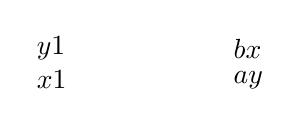
\begin{tikzpicture}[scale = 1, transform shape]
    \storageTwoThreads
    \node[right] at (1, -0.2) {\storageFont $\writeInst{x}{1}$};
    \node[right] at (1,  0.2) {\storageFont $\writeInst{y}{1}$};
    \node[right] at (3.5, -0.2) {\storageFont $\readInst{a}{y}$};
    \node[right] at (3.5,  0.2) {\storageFont $\readInst{b}{x}$};
  \end{tikzpicture}
  \caption{}
  \label{fig:armvpop:mpstorage:1}
\end{subfigure}%
\begin{subfigure}{.33\textwidth}
  \begin{tikzpicture}[scale = 1, transform shape]
    \storageTwoThreads
    \node[right] at (1,  0) {\storageFont $\writeInst{x}{1}$};
    \node[right] at (2.25, -1.6) {\storageFont $\writeInst{y}{1}$};
    \node[right] at (2.25, -1.2) {\storageFont $\readInst{a}{y}$};
    \node[right] at (2.25, -0.8) {\storageFont $\readInst{b}{x}$};
  \end{tikzpicture}
  \caption{}
  \label{fig:armvpop:mpstorage:2}
\end{subfigure}%
\begin{subfigure}{.33\textwidth}
  \begin{tikzpicture}[scale = 1, transform shape]
    \storageTwoThreads
    \node[right] at (1,  0) {\storageFont $\writeInst{x}{1}$};
    \node[right] at (2.25, -1.4) {\storageFont $\writeInst{y}{1}$};
    \node[right] at (2.25, -1) {\storageFont $\readInst{b}{x}$};
  \end{tikzpicture}
  \caption{}
  \label{fig:armvpop:mpstorage:3}
\end{subfigure}
\caption{Состояние подсистемы памяти ARMv8 POP при исполнении программы ${\rm MP}$}
\label{fig:armvpop:mpstorage}
\end{figure}

Результат $[a = 1, b = 0]$ в ARM машине может быть получен двумя способами.
Во-первых, подсистема управления имеет право исполнять инструкции не по порядку (out-of-order execution).
Так, первый поток в программе ${\rm MP}$ может отправить запрос на запись $\writeInst{y}{1}$ в подсистему памяти до запроса $\writeInst{x}{1}$,
соответственно второй поток может увидеть эти запросы в отличном от программного порядке.
Во-вторых, подсистема памяти также может переупорядочить запросы внутри себя.
Так, сначала оба потока отправляют по два запроса в подсистему памяти (см. рис. \ref{fig:armvpop:mpstorage:1}).
После подсистема переупорядочивает независимые запросы $\writeInst{x}{1}$ и $\writeInst{y}{1}$, отправляет $\writeInst{y}{1}$
в общий для двух потоков буфер, как и запросы второго потока (см. рис. \ref{fig:armvpop:mpstorage:2}).
Поскольку в общем буфере запросы $\writeInst{y}{1}$ и $\readInst{a}{y}$ находятся рядом, то подсистема памяти может послать
ответ $[a \leftarrow 1]$ на запрос $\readInst{a}{y}$ в подсистему управления (cм. рис. \ref{fig:armvpop:mpstorage:3}).
После чего запрос $\writeInst{x}{1}$ отправляется в общий буфер, а затем все оставшиеся запросы в отправляются в память,
что приводит к результату $[a = 1, b = 0]$.

В разделе \ref{sec:overview:effcompl} было сказано, что аналогичный сценарий поведения в случае архитектуры Power может быть запрещен
с помощью барьеров памяти. Это верно и для модели ARMv8 POP. Так, следующая программа не имеет сценария поведения с результатом $[a = 1, b = 0]$:
\begin{equation*}
\tag{MP-SY-LD}\label{ex:MP-sy-ld}
\begin{tabular}{c}
  $\writeInst{x}{0}; \writeInst{y}{0};$ \\
\begin{tabular}{L || L}
  \writeInst{x}{1};  & \readInst{a}{y}; ~\valueneg{1} \\
  \dmbSY; & \dmbLD; \\
  \writeInst{y}{1}  & \readInst{b}{x} ~\valueneg{0} \\
\end{tabular}
\end{tabular}
\end{equation*}
\emph{Полный барьер} $\dmbSY$ в первом потоке заставляет подсистему управления отправить все три запроса в исходном порядке;
кроме того, запрос, соответствующий полному барьеру, не может быть переупорядочен с другими запросами внутри
подсистемы памяти%
\footnote{Вместо полного барьера в этой программе мог бы быть использован \emph{барьер на запись} $\dmbST$,
однако барьер на запись не соответствует ни одной конструкции в обещающей модели, так же как и в оригинальной модели C/C++11.}.
Так, барьер $\dmbSY$ гарантирует, что запрос $\writeInst{y}{1}$ попадает в общий буфер подсистемы памяти только после $\writeInst{x}{1}$.
Во втором потоке \emph{барьер на чтение} $\dmbLD$ запрещает подсистеме управления отправлять запрос на чтение $\readInst{b}{x}$ до того
момента, пока она не получит ответ на запрос $\readInst{a}{y}$.
Таким образом гарантируется, что если $a = 1$, то $b = 1$.

В приведенных сценариях поведения было важно, что подсистема памяти может переупорядочивать лишь некоторые пары сообщений.
Какие пары могут быть переупорядочены, а какие нет определяется отношением $\reorderableRel{\e_{\rm old}}{\e_{\rm new}}$:
\begin{definition}
Запросы $\e_{\rm old}$ и $\e_{\rm new}$ могут быть \emph{переупорядочены}, что обозначается $\reorderableRel{\e_{\rm old}}{\e_{\rm new}}$,
если среди них нет полного барьера, и они оперируют над разными локациями.
\end{definition}

Отметим, что в этом доказательстве мы рассматриваем ослабленную, т.е. допускающую большее число сценариев поведения, версию
модели ARMv8 POP \cite{Flur-al:POPL16}, в которой подсистема управления не отсылает запросы, соответствующие барьеру $\dmbLD$,
в подсистему памяти%
\footnote{
  Почему рассмотренная модель допускает большее число поведений?
  Предположим, что модель посылает $\dmbLD$ запросы в память, но они
  могут быть переупорядочены со всеми остальными.
  Такая модель, очевидно, допускает больше сценариев поведения, чем оригинальная, накладывающая ограничения на
  переупорядочивание с $\dmbLD$. Так же очевидно, что полученная модель допускает те же сценарии, что и модель, которая
  не посылает $\dmbLD$ запросы.
}.
Поскольку нам удалось доказать корректность компиляции для ослабленной версии модели, то корректность компиляции сохраняется
и для изначальной модели.

Теперь рассмотрим сценарий поведения программы ${\rm ARM\text{-}weak}$,
в котором получается результат $[a = 1]$:
\begin{equation*}
\tag{ARM-weak}
\begin{tabular}{c}
  $\writeInst{x}{0}; \writeInst{y}{0};$ \\
\begin{tabular}{L || L || L}
  \readInst{a}{x}; \; \valuecom{1} & \readInst{b}{x}; & \readInst{c}{y}; \\
  \writeInst{x}{1}                 & \writeInst{y}{b} & \writeInst{x}{c} \\
\end{tabular}
\end{tabular}
\end{equation*}
Такой результат получается в модели ARMv8 POP, если у первого и второго потоков
есть общий буфер, который не виден третьему потоку.
Для получения результата $[a = 1]$ первый поток отправляет оба запроса,
на чтение $\readInst{a}{x}$ и на запись $\writeInst{x}{1}$,
в подсистему памяти, а второй поток также отправляет запрос на чтение $\readInst{b}{x}$,
после чего все запросы попадают в общий для первого и второго потоков буфер
(см. рис. \ref{fig:armvpop:armweakstorage:1}).
Поскольку запросы на чтение $\readInst{b}{x}$ и на запись $\writeInst{x}{1}$
находятся в одном буфере, и ближе к основной памяти находится запрос на запись,
то подсистема памяти может послать ответ $[b \leftarrow 1]$ второму потоку,
а сам поток после этого --- послать запрос $\writeInst{y}{1}$, который
через общий буфер и переупорядочивание с запросами о локации $x$ в нём
попадает в основную память
(см. рис. \ref{fig:armvpop:armweakstorage:2}). 
Теперь третий поток посылает запрос на чтение $\readInst{c}{y}$
(см. рис. \ref{fig:armvpop:armweakstorage:3}), который разрешается в общей памяти
с ответом $[c \leftarrow 1]$.
После чего третий поток посылает запрос на запись $\writeInst{x}{1}$
(см. рис. \ref{fig:armvpop:armweakstorage:4}), который далее используется для
отправки ответа на запрос чтения $\readInst{a}{x}$, приводя к результату $[a = 1]$.

\begin{figure}
\begin{subfigure}{.5\textwidth}
\begin{center}
\begin{tikzpicture}[scale = 1, transform shape]
    \storageThreeThreads
    \node[right] at (2.25, -0.4) {\storageFont $\readInst{b}{x}$};
    \node[right] at (2.25, -0.8) {\storageFont $\writeInst{x}{1}$};
    \node[right] at (2.25, -1.2) {\storageFont $\readInst{a}{x}$};
    \node at (4.125, -2.7) {\storageFont $\writeInst{x}{0}; \writeInst{y}{0}$};
\end{tikzpicture}
  \caption{}
  \label{fig:armvpop:armweakstorage:1}
\end{center}
\end{subfigure}%
\begin{subfigure}{.5\textwidth}
\begin{center}
\begin{tikzpicture}[scale = 1, transform shape]
    \storageThreeThreads
    \node[right] at (2.25, -0.6) {\storageFont $\writeInst{x}{1}$};
    \node[right] at (2.25, -1) {\storageFont $\readInst{a}{x}$};
    \node at (4.125, -2.7) {\storageFont $\writeInst{x}{0}; \writeInst{y}{1}$};
\end{tikzpicture}
  \caption{}
  \label{fig:armvpop:armweakstorage:2}
\end{center}
\end{subfigure}

\begin{subfigure}{.5\textwidth}
\begin{center}
\begin{tikzpicture}[scale = 1, transform shape]
    \storageThreeThreads
    \node[right] at (2.25, -0.6) {\storageFont $\writeInst{x}{1}$};
    \node[right] at (2.25, -1) {\storageFont $\readInst{a}{x}$};
    \node[right] at (4.125, -1.8) {\storageFont $\readInst{c}{y}$};
    \node at (4.125, -2.7) {\storageFont $\writeInst{x}{0}; \writeInst{y}{1}$};
\end{tikzpicture}
  \caption{}
  \label{fig:armvpop:armweakstorage:3}
\end{center}
\end{subfigure}%
\begin{subfigure}{.5\textwidth}
\begin{center}
\begin{tikzpicture}[scale = 1, transform shape]
    \storageThreeThreads
    \node[right] at (2.25, -0.6) {\storageFont $\writeInst{x}{1}$};
    \node[right] at (2.25, -1) {\storageFont $\readInst{a}{x}$};
    \node[right] at (4.125, -1.8) {\storageFont $\writeInst{x}{1}$};
    \node at (4.125, -2.7) {\storageFont $\writeInst{x}{0}; \writeInst{y}{1}$};
\end{tikzpicture}
  \caption{}
  \label{fig:armvpop:armweakstorage:4}
\end{center}
\end{subfigure}
\caption{Состояние подсистемы памяти ARMv8 POP при исполнении программы
  ${\rm ARM\text{-}weak}$}
\label{fig:armvpop:armweakstorage}
\end{figure}

\subsection{Абстрактная подсистема памяти: POP}
В \cite{Flur-al:POPL16} подсистема памяти модели ARM представлена в двух вариантах:
Flowing и POP (partial order propagation).
Несмотря на то, что мы называем модель из \cite{Flur-al:POPL16} моделью ARMv8 POP,
до этого момента в примерах мы использовали подсистему памяти Flowing, поскольку
она нагляднее.
Тем не менее, у Flowing есть два ключевых недостатка, которые решаются POP ---
более абстрактным вариантом подсистемы памяти.
Во-первых, вместо того, чтобы представлять буфер как список запросов и
рассматривать перестановки в нём, математически удобнее представлять его как
частично упорядоченное множество.
Во-вторых, подсистема Flowing требует введения конкретной топологии буферов,
что при рассуждениях о всех сценариях поведения программы заставляет
дополнительно рассматривать и варианты топологий.

В подсистеме POP нет линейных буферов и фиксированной топологии.
Вместо этого состояние подсистемы представляется как тройка
$\angled{\Evt, \Ord, \Prop}$, где
$\Evt$ --- это множество текущих запросов в подсистеме,
$\Ord$ --- это частичный порядок на запросах из $\Evt$, а
$\Prop$ --- это функция, которая по идентификатору потока возвращает
множество ``распространённых'' на поток запросов.
Если запросы $\e$ и $\e'$ упорядочены отношением $\Ord$, т.е. $\Ord(\e, \e')$,
то мы пишем $\e <_{\Ord} \e'$.

Для того, чтобы понять, как подсистема POP работает и соотносится с подсистемой Flowing,
мы рассмотрим слабый сценарий поведения следующей программы с результатом $[a = 1, b = 1, c = 0]$:
\begin{equation*}
\tag{WRC-data-addr}\label{ex:WRC+data+addr}
\begin{tabular}{L || Ll || Ll}
\writeInst{x}{1}; & \readInst{a}{x};  & \valuecom{1} & \readInst{b}{y}; & \valuecom{1} \\
                  & \writeInst{y}{a}  &              & \readInst{c}{x + b * 0} & \valuecom{0}  \\
\end{tabular}
\end{equation*}
В данной программе подсистема управления модели ARMv8 POP во втором и третьем потоках
не может отправить запросы, относящиеся ко второй строчке, пока не получит ответ на первые
инструкции, поскольку во втором потоке между инструкциями существует зависимость по данным,
а в третьем --- мнимая (fake) зависимость по адресу.
Таким образом, эффект слабого сценария поведения в ARMv8 POP должен быть получен за счёт
подсистемы памяти. 

\begin{figure}
  \begin{subfigure}{.5\textwidth}
\begin{center}
\begin{tikzpicture}[baseline=-20pt,scale = 1, transform shape]
  \storageThreeThreadsWRC
  \node[right] at (1  ,  0) {\storageFont $m: \writeInst{x}{1}$};
  \node[right] at (3.5,  0) {\storageFont $n: \readInst{a}{x}$};
  \node[right] at (6  ,  0) {\storageFont $o: \readInst{b}{y}$};
  \node at (4.125, -2.7) {\storageFont $k: \writeInst{x}{0}; \; l: \writeInst{y}{0}$};
\end{tikzpicture}
\end{center}
    \caption{}
    \label{fig:armvpop:flpop:1}
  \end{subfigure}%
  \begin{subfigure}{.5\textwidth}
\begin{center}
\parbox{63mm}{$\begin{array}{@{}r@{~}l@{}}
  \Evt      &= \{k, l, m, n, o\} \\
  \Ord      &= \{ (k, m), (k, n), (l, o) \} \\
  \Prop(T1) &= \{k, l, m\} \\
  \Prop(T2) &= \{k, l, n\} \\
  \Prop(T3) &= \{k, l, o\} \\
\end{array}$}
\end{center}
    \caption{}
    \label{fig:armvpop:flpop:2}
  \end{subfigure}
  \hrule

  \begin{subfigure}{.5\textwidth}
\begin{center}
\begin{tikzpicture}[baseline=-20pt,scale = 1, transform shape]
    \storageThreeThreadsWRC
    \node[right] at (2.25, -1.0) {\storageFont $m: \writeInst{x}{1}$};
    \node[right] at (3.5 ,    0) {\storageFont $n: \readInst{a}{x}$};
    \node[right] at (6    ,   0) {\storageFont $o: \readInst{b}{y}$};
    \node at (4.125, -2.7) {\storageFont $k: \writeInst{x}{0}; \; l: \writeInst{y}{0}$};
\end{tikzpicture}
\end{center}
    \caption{}
    \label{fig:armvpop:flpop:3}
  \end{subfigure}%
  \begin{subfigure}{.5\textwidth}
\begin{center}
\parbox{63mm}{$\begin{array}{@{}r@{~}l@{}}
  \Evt      &= \{k, l, m, n, o\} \\
  \Ord      &= \{ (k, m), (k, n), \\
            & ~~\quad (l, o), \graybox{(m, n)} \} \\
  \Prop(T1) &= \{k, l, m\} \\
  \Prop(T2) &= \{k, l, n, \graybox{m}\} \\
  \Prop(T3) &= \{k, l, o\} \\
\end{array}$}
\end{center}
    \caption{}
    \label{fig:armvpop:flpop:4}
  \end{subfigure}
  \hrule

  \begin{subfigure}{.5\textwidth}
\begin{center}
\begin{tikzpicture}[baseline=-20pt,scale = 1, transform shape]
    \storageThreeThreadsWRC
    \node[right] at (2.25, -1.2) {\storageFont $m: \writeInst{x}{1}$};
    \node[right] at (2.25, -0.8) {\storageFont $n: \readInst{a}{x}$};
    \node[right] at (6    ,   0) {\storageFont $o: \readInst{b}{y}$};
    \node at (4.125, -2.7) {\storageFont $k: \writeInst{x}{0}; \; l: \writeInst{y}{0}$};
\end{tikzpicture}
\end{center}
    \caption{}
    \label{fig:armvpop:flpop:5}
  \end{subfigure}%
  \begin{subfigure}{.5\textwidth}
\begin{center}
\parbox{63mm}{$\begin{array}{@{}r@{~}l@{}}
  \Evt      &= \{k, l, m, n, o\} \\
  \Ord      &= \{ (k, m), (k, n), \\
            & ~~\quad (l, o), (m, n) \} \\
  \Prop(T1) &= \{k, l, m, \graybox{n} \} \\
  \Prop(T2) &= \{k, l, n, m\} \\
  \Prop(T3) &= \{k, l, o\} \\
\end{array}$}
\end{center}
    \caption{}
    \label{fig:armvpop:flpop:6}
  \end{subfigure}
  \caption{Состояние подсистем Flowing и POP при исполнении программы ${\rm WRC\text{-}data\text{-}addr}$}
\end{figure}
\begin{figure}\ContinuedFloat
  \begin{subfigure}{.5\textwidth}
\begin{center}
\begin{tikzpicture}[baseline=-20pt,scale = 1, transform shape]
    \storageThreeThreadsWRC
    \node[right] at (2.25, -1.0) {\storageFont $m: \writeInst{x}{1}$};
    \node[right] at (3.5,     0) {\storageFont $p: \writeInst{y}{1}$};
    \node[right] at (6    ,   0) {\storageFont $o: \readInst{b}{y}$};
    \node at (4.125, -2.7) {\storageFont $k: \writeInst{x}{0}; \; l: \writeInst{y}{0}$};
\end{tikzpicture}
\end{center}
    \caption{}
    \label{fig:armvpop:flpop:7}
  \end{subfigure}%
  \begin{subfigure}{.5\textwidth}
\begin{center}
\parbox{63mm}{$\begin{array}{@{}r@{~}l@{}}
  \Evt      &= \{k, l, m, o, \graybox{p}\} \\
  \Ord      &= \{ (k, m), (l, o), \graybox{(l, p)} \} \\
  \Prop(T1) &= \{k, l, m\} \\
  \Prop(T2) &= \{k, l, m, \graybox{p}\} \\
  \Prop(T3) &= \{k, l, o\} \\
\end{array}$}
\end{center}
    \caption{}
    \label{fig:armvpop:flpop:8}
  \end{subfigure}
  \hrule

  \begin{subfigure}{.5\textwidth}
\begin{center}
\begin{tikzpicture}[baseline=-20pt,scale = 1, transform shape]
    \storageThreeThreadsWRC
    \node[right] at (2.25, -1.0) {\storageFont $m: \writeInst{x}{1}$};
    \node[right] at (6    ,   0) {\storageFont $o: \readInst{b}{y}$};
    \node at (4.125, -2.7) {\storageFont $k: \writeInst{x}{0}; \; p: \writeInst{y}{1}$};
\end{tikzpicture}
\end{center}
    \caption{}
    \label{fig:armvpop:flpop:9}
  \end{subfigure}%
  \begin{subfigure}{.5\textwidth}
\begin{center}
\parbox{63mm}{$\begin{array}{@{}r@{~}l@{}}
  \Evt      &= \{k, l, m, o, p\} \\
  \Ord      &= \{ (k, m), (l, o), \\
            & ~~\quad (l, p), \graybox{(p, o)} \} \\
  \Prop(T1) &= \{k, l, m, \graybox{p}\} \\
  \Prop(T2) &= \{k, l, m, p\} \\
  \Prop(T3) &= \{k, l, o, \graybox{p}\} \\
\end{array}$}
\end{center}
    \caption{}
    \label{fig:armvpop:flpop:10}
  \end{subfigure}
  \hrule

  \begin{subfigure}{.5\textwidth}
\begin{center}
\begin{tikzpicture}[baseline=-20pt,scale = 1, transform shape]
    \storageThreeThreadsWRC
    \node[right] at (2.25, -1.0) {\storageFont $m: \writeInst{x}{1}$};
    \node[right] at (6    ,   0) {\storageFont \phantom{$o: \readInst{b}{y}$}};
    \node[right] at (4.125,  -2) {\storageFont $o: \readInst{b}{y}$};
    \node at (4.125, -2.7) {\storageFont $k: \writeInst{x}{0}; \; p: \writeInst{y}{1}$};
\end{tikzpicture}
\end{center}
    \caption{}
    \label{fig:armvpop:flpop:11} 
  \end{subfigure}%
  \begin{subfigure}{.5\textwidth}
\begin{center}
\parbox{63mm}{$\begin{array}{@{}r@{~}l@{}}
  \Evt      &= \{k, l, m, o, p\} \\
  \Ord      &= \{ (k, m), (l, o), \\
            & ~~\quad (l, p), (p, o) \} \\
  \Prop(T1) &= \{k, l, m, p, \graybox{o}\} \\
  \Prop(T2) &= \{k, l, m, p, \graybox{o}\} \\
  \Prop(T3) &= \{k, l, o, p\} \\
\end{array}$}
\end{center}
    \caption{}
    \label{fig:armvpop:flpop:12}
  \end{subfigure}

  \caption{Состояние подсистем Flowing и POP при исполнении программы ${\rm WRC\text{-}data\text{-}addr}$ (продолжение)}
  \label{fig:armvpop:flpop}
\end{figure}

Для того, чтобы воспроизвести упомянутый результат, в рамках подсистемы Flowing нужно
выбрать такую же топологию буферов, как и для слабого сценария поведения программы
${\rm ARM\text{-}weak}$: должен быть буфер, общий для первого и второго потоков.

Пусть все три потока отправили по одному запросу в подсистему памяти.
Соответствующие состояния Flowing и POP представлены на
рис. \ref{fig:armvpop:flpop:1} и \ref{fig:armvpop:flpop:2}.
Заметим, что для краткости мы помечаем запросы в Flowing буквенными
идентификаторами и используем их в описании состояния POP.

Когда поток $T$ отправляет запрос $\e$ в подсистему памяти POP,
во множество $\Ord$ добавляется по ребру $(\e', \e)$
за каждый запрос $\e'$, о котором поток $T$ осведомлён, т.е.
$\e' \in \Prop(T)$, и который также не может быть переупорядочен с $\e$,
т.е. $\notReorderableRel{\e'}{\e}$.
Поэтому на рис. \ref{fig:armvpop:flpop:2} отношение $\Ord$ не пусто ---
в нём присутствуют ребра, связывающие отправленные потоками запросы
с инициализирующими записями в локации.

Далее подсистема памяти может перенести запрос $m: \writeInst{x}{1}$ в общий
для первого и второго потоков буфер. В терминах подсистемы POP это означает,
что второй поток становится осведомлённым об этом запросе
(см. рис. \ref{fig:armvpop:flpop:3} и \ref{fig:armvpop:flpop:4}).
Запрос $m$ попадает во множество $\Prop(T2)$, а в отношение $\Ord$ добавляется
ребро $(m, n)$.

В общем случае, когда поток $T'$ становится осведомлённым о запросе $\e$ потока $T$,
т.е., в терминах Flowing, $\e$ попадает в видимый для $T'$ буфер,
или, в терминах POP, $\e$ становится элементом $\Prop(T')$, то
подсистема POP добавляет по ребру $(\e, \e')$ во множество $\Ord$
за каждый запрос $\e' \in \Prop(T') \setminus \Prop(T)$, если
запросы не могут быть переупорядочены, т.е. $\notReorderableRel{\e}{\e'}$,
и между ними нет обратного ребра $(\e', \e)$ в отношении $\Ord$.
В рассматриваемом сценарии поведения программы ${\rm WRC\text{-}data\text{-}addr}$
запросы $m$ и $n$ не переупорядочиваемы, т.к. они оперируют над одной и той же локацией $x$,
поэтому на рис. \ref{fig:armvpop:flpop:4} между ними появляется $\Ord$-ребро.

Далее запрос $n$ попадает в общий для первого и второго потоков буфер
(подсистема Flowing, рис. \ref{fig:armvpop:flpop:5}), что
соответствует тому, что первый поток становится осведомлённым о запросе $n$
(подсистема POP, рис. \ref{fig:armvpop:flpop:6}).
Теперь запрос $n : \readInst{a}{x}$ непосредственно следует за запросом $m : \writeInst{x}{1}$
в общем для первого и второго потоков буфере (подсистема Flowing),
о запросах осведомлены одни и те же потоки, и между ними нет никакого запроса в отношении $\Ord$
(подсистема POP).
Это означает, что и Flowing, и POP могут отправить ответ $[n \leftarrow 1]$ на запрос $n: \readInst{a}{x}$.
После получения ответа второй поток отправляет запрос $p: \writeInst{y}{1}$ в подсистему памяти
(см. рис. \ref{fig:armvpop:flpop:7} и \ref{fig:armvpop:flpop:8}).
Далее подсистема памяти отправляет запрос $p: \writeInst{y}{1}$ в общий буфер и в основную память
(см. рис. \ref{fig:armvpop:flpop:9}, подсистема Flowing), и делает первый и третий потоки
осведомлёнными о нём
(см. рис. \ref{fig:armvpop:flpop:10}, подсистема POP).
Заметим, что поскольку в подсистеме POP нет фиксированной топологии буферов, подсистема может
осведомить первый поток о запросе $p$, а потом --- третий поток, или наоборот.

Теперь запрос $o: \readInst{b}{y}$ может попасть в общий для всех потоков буфер
(см. рис. \ref{fig:armvpop:flpop:11} и \ref{fig:armvpop:flpop:12}) и, затем, в память, что
приведёт к отправке ответа $[b \leftarrow 1]$ на него.
После этого третий поток посылает запрос $\readInst{c}{x}$, который, попав в основную память,
получает ответ $[c \leftarrow 0]$.
В конце сценария поведения запрос $m : \writeInst{x}{1}$ попадает в память.
Так, мы получили результат $[a = 1, b = 1, c = 0]$.

В конце исполнения программы в модели ARMv8 POP с подсистемой POP все выпущенные запросы записи и барьеров
памяти попадают в основную память, и, соответственно, все потоки становятся осведомлёнными о них.
Как следствие, все записи в одну локацию тотально упорядочены отношением $\Ord$.
В рамках описанного ниже доказательства корректности компиляции мы используем этот порядок для введения меток времени
на запросах записи в подсистеме памяти.

Поскольку в \cite{Flur-al:POPL16} доказано, что подсистема POP допускает все сценарии поведения, возможные с подсистемой Flowing,
и кроме того является более абстрактной, то мы используем именно её в своём доказательстве.

\subsection{Обещающая модель}

Как уже было отмечено в этой главе, обещающая модель памяти, аналогично модели $\OpCpp$, использует
метки времени, базовые фронты и фронты сообщений.
Так, слабый сценарий поведения программы ${\rm MP}$, имеющий результат $[a = 1, b = 0]$, имеет
абсолютно ту же структуру в обещающей модели, что и в модели $\OpCpp$.
Кратко проиллюстрируем его. 
\begin{equation*}
\tag{MP}
\begin{tabular}{c}
  $\writeInst{x}{0}; \writeInst{y}{0};$ \\
\begin{tabular}{L || L}
  \writeInst{x}{1}; & \readInst{a}{y}; ~\valuecom{1} \\
  \writeInst{y}{1} & \readInst{b}{x}~ ~\valuecom{0} \\
\end{tabular}
\end{tabular}
\end{equation*}
После исполнения инициализирующих записей и старта потоков память и базовые фронты потоков имеют следующие значения:
\[
\begin{array}{l}
M = \{\angled{x:0@\tstamp{0}, [x@\tstamp{0}]}, \angled{y:0@\tstamp{0}, [y@\tstamp{0}]}\}; \\
T1.\Rcur = [x@\tstamp{0}, y@\tstamp{0}];
\quad T2.\Rcur = [x@\tstamp{0}, y@\tstamp{0}].
\end{array}
\]
После того, как левый поток выполняет обе записи, в памяти появляются два новых сообщения
и базовый фронт первого потока обновляется соответствующим образом:
\[
\begin{array}{l}
M = \{\angled{x:0@\tstamp{0}, [x@\tstamp{0}]}, \angled{y:0@\tstamp{0}, [x@\tstamp{0}]},\\
\quad \quad \quad \graybox{\angled{x:1@\tstamp{1}, [x@\tstamp{1}, y@\tstamp{0}]}}, \graybox{\angled{y:1@\tstamp{1}, [x@\tstamp{0}, y@\tstamp{1}]}}\}; \\
T1.\Rcur = [x@\graybox{\tstamp{1}}, y@\graybox{\tstamp{1}}]; \quad T2.\Rcur = [x@\tstamp{0}, y@\tstamp{0}].
\end{array}
\]
Теперь второй поток может прочитать новое сообщение $\angled{y:1@\tstamp{1}, [x@\tstamp{0}, y@\tstamp{1}]}$ и
старое сообщение $\angled{x:1@\tstamp{1}, [x@\tstamp{1}, y@\tstamp{0}]}$, что приводит к результату $[a = 1, b = 0]$.

Рассмотрим то, как слабый сценарий поведения с результатом $[a = 1, b = 0]$ программы ${\rm MP\text{-}SY\text{-}LD}$
запрещается в обещающей модели.
\begin{equation*}
\tag{MP-SY-LD}\label{ex:MP-sy-ld}
\begin{tabular}{c}
  $\writeInst{x}{0}; \writeInst{y}{0};$ \\
\begin{tabular}{L || L}
  \writeInst{x}{1}; & \readInst{a}{y}; ~\valueneg{1} \\
  \dmbSY;           & \dmbLD; \\
  \writeInst{y}{1}  & \readInst{b}{x} ~\valueneg{0} \\
\end{tabular}
\end{tabular}
\end{equation*}
В рассматриваемой нами схеме компиляции барьеры $\dmbSY$ и $\dmbLD$ являются результатами компиляции
высвобождающего и приобретающего барьеров соответственно.
Для их поддержки в обещающей модели используются высвобождающий ($\Rrel$) и приобретающий ($\Racq$)
фронты потоков.
Последний аналогичен приобретающему фронту из модели $\OpCpp$.

После выполнения инициализирующих записей и старта потоков конфигурация абстрактной машины, реализующей
обещающую модель, далее \emph{обещающая машина}, или \emph{машина \Promise}, выглядит следующим образом:
\[
\begin{array}{l l l}
\multicolumn{3}{l}{M = \{\angled{x:0@\tstamp{0}, [x@\tstamp{0}]}, \angled{y:0@\tstamp{0}, [y@\tstamp{0}]}\}; } \\
T1.\Rcur = [x@\tstamp{0}, y@\tstamp{0}]; & 
T1.\Racq = [x@\tstamp{0}, y@\tstamp{0}]; & 
T1.\Rrel = [x@\tstamp{0}, y@\tstamp{0}];           \\
T2.\Rcur = [x@\tstamp{0}, y@\tstamp{0}]; &
T2.\Racq = [x@\tstamp{0}, y@\tstamp{0}]; &
T2.\Rrel = [x@\tstamp{0}, y@\tstamp{0}]. \\
\end{array}
\]
После того, как первый поток выполняет запись $\writeInst{x}{1}$, в память добавляется новое сообщение,
а базовый и приобретающий фронты потока обновляются на соответствующую метку времени:
\[
\begin{array}{l l l}
\multicolumn{3}{l}{M = \{\angled{x:0@\tstamp{0}, [x@\tstamp{0}]}, \angled{y:0@\tstamp{0}, [y@\tstamp{0}]},
  \graybox{\angled{x:1@\tstamp{1}, [x@\tstamp{1}, y@\tstamp{0}]}} \}; } \\
T1.\Rcur = [x@\graybox{\tstamp{1}}, y@\tstamp{0}]; & 
T1.\Racq = [x@\graybox{\tstamp{1}}, y@\tstamp{0}]; & 
T1.\Rrel = [x@\tstamp{0}, y@\tstamp{0}];           \\
T2.\Rcur = [x@\tstamp{0}, y@\tstamp{0}]; &
T2.\Racq = [x@\tstamp{0}, y@\tstamp{0}]; &
T2.\Rrel = [x@\tstamp{0}, y@\tstamp{0}]. \\
\end{array}
\]
При этом фронтом сообщения становится высвобождающий фронт $\Rrel$ первого потока, увеличенный на метку времени
самого сообщения по целевой локации.

После того, как первый фронт выполняет высвобождающий барьер, который в программе представлен его скомпилированным
вариантом $\dmbSY$, высвобождающий фронт $\Rrel$ потока становится равен базовому фронту потока:
\[
\begin{array}{l l l}
\multicolumn{3}{l}{M = \{\angled{x:0@\tstamp{0}, [x@\tstamp{0}]}, \angled{y:0@\tstamp{0}, [y@\tstamp{0}]},
  \angled{x:1@\tstamp{1}, [x@\tstamp{1}, y@\tstamp{0}]} \};} \\
T1.\Rcur = [x@\tstamp{1}, y@\tstamp{0}];           &
T1.\Racq = [x@\tstamp{1}, y@\tstamp{0}];           &
T1.\Rrel = [x@\graybox{\tstamp{1}}, y@\tstamp{0}]; \\
T2.\Rcur = [x@\tstamp{0}, y@\tstamp{0}]; &
T2.\Racq = [x@\tstamp{0}, y@\tstamp{0}]; &
T2.\Rrel = [x@\tstamp{0}, y@\tstamp{0}]. \\
\end{array}
\]
После этого первый поток выполняет вторую запись по тем же правилам, что и первую:
\[
\begin{array}{l l l}
\multicolumn{3}{l}{M = \{\angled{x:0@\tstamp{0}, [x@\tstamp{0}]}, \angled{y:0@\tstamp{0}, [y@\tstamp{0}]},} \\
\multicolumn{3}{l}{
\quad \quad \quad \angled{x:1@\tstamp{1}, [x@\tstamp{1}, y@\tstamp{0}]}, \graybox{\angled{y:1@\tstamp{1}, [x@\tstamp{1}, y@\tstamp{1}]}} \};} \\
T1.\Rcur = [x@\tstamp{1}, y@\graybox{\tstamp{1}}]; &
T1.\Racq = [x@\tstamp{1}, y@\graybox{\tstamp{1}}]; &
T1.\Rrel = [x@\tstamp{1}, y@\tstamp{0}]; \\
T2.\Rcur = [x@\tstamp{0}, y@\tstamp{0}]; &
T2.\Racq = [x@\tstamp{0}, y@\tstamp{0}]; &
T2.\Rrel = [x@\tstamp{0}, y@\tstamp{0}]. \\
\end{array}
\]
Теперь второй поток может выполнить чтение из добавленного сообщения, получая $[a = 1]$.
При этом базовый фронт потока $\Rcur$ обновляется на $[y@\tstamp{1}]$, а приобретающий $\Racq$ --- на фронт сообщения,
$[x@\tstamp{1}, y@\tstamp{1}]$, как это было и в модели $\OpCpp$:
\[
\begin{array}{l l l}
\multicolumn{3}{l}{M = \{\angled{x:0@\tstamp{0}, [x@\tstamp{0}]}, \angled{y:0@\tstamp{0}, [y@\tstamp{0}]},} \\
\multicolumn{3}{l}{
\quad \quad \quad \angled{x:1@\tstamp{1}, [x@\tstamp{1}, y@\tstamp{0}]}, \angled{y:1@\tstamp{1}, [x@\tstamp{1}, y@\tstamp{1}]} \};} \\
T1.\Rcur = [x@\tstamp{1}, y@\tstamp{1}]; &
T1.\Racq = [x@\tstamp{1}, y@\tstamp{1}]; &
T1.\Rrel = [x@\tstamp{1}, y@\tstamp{0}]; \\
T2.\Rcur = [x@\tstamp{0}, y@\tstamp{0}]; &
T2.\Racq = [x@\graybox{\tstamp{1}}, y@\graybox{\tstamp{1}}]; &
T2.\Rrel = [x@\tstamp{0}, y@\tstamp{0}]. \\
\end{array}
\]
После выполнения приобретающего барьера, который в программе представлен его скомпилированным вариантом $\dmbLD$,
базовый фронт $\Rcur$ второго потока становится равным приобретающему фронту $\Racq$:
\[
\begin{array}{l l l}
\multicolumn{3}{l}{M = \{\angled{x:0@\tstamp{0}, [x@\tstamp{0}]}, \angled{y:0@\tstamp{0}, [y@\tstamp{0}]},} \\
\multicolumn{3}{l}{
\quad \quad \quad \angled{x:1@\tstamp{1}, [x@\tstamp{1}, y@\tstamp{0}]}, \angled{y:1@\tstamp{1}, [x@\tstamp{1}, y@\tstamp{1}]} \};} \\
T1.\Rcur = [x@\tstamp{1}, y@\tstamp{1}]; &
T1.\Racq = [x@\tstamp{1}, y@\tstamp{1}]; &
T1.\Rrel = [x@\tstamp{1}, y@\tstamp{0}]; \\
T2.\Rcur = [x@\graybox{\tstamp{1}}, y@\graybox{\tstamp{1}}] &
T2.\Racq = [x@\tstamp{1}, y@\tstamp{1}]; &
T2.\Rrel = [x@\tstamp{0}, y@\tstamp{0}]. \\
\end{array}
\]
Теперь второй поток не может прочитать старое сообщение $\angled{x:0@\tstamp{0}, [x@\tstamp{0}]}$, т.к.
$T2.\Rcur(x) = \tstamp{1} > \tstamp{0}$. Таким образом, результат $[a = 1, b = 0]$ запрещается.

Перейдем к рассмотрению слабого сценария поведения программы ${\rm ARM\text{-}weak}$ с результатом $[a = 1, b = 1, c = 1]$
в обещающей модели%
\footnote{Стоит отметить, что такой результат для программы ${\rm ARM\text{-}weak}$ невозможен в модели $\OpCpp$,
  но возможен в оригинальной модели C/C++11.}.
\begin{equation*}
\tag{ARM-weak}
\begin{tabular}{c}
  $\writeInst{x}{0}; \writeInst{y}{0};$ \\
\begin{tabular}{L || L || L}
  \readInst{a}{x}; \; \valuecom{1} & \readInst{b}{x}; & \readInst{c}{y}; \\
  \writeInst{x}{1}                 & \writeInst{y}{b} & \writeInst{x}{c} \\
\end{tabular}
\end{tabular}
\end{equation*}

Для того, чтобы получить интересующий результат для этой программы, обещающая модель, в соответствии со своим названием,
использует \emph{механизм обещаний}
Так, в любой момент исполнения поток может сделать одно из двух действий:
либо выполнить следующую инструкцию, либо \emph{пообещать} сделать некоторую запись в будущем.
Когда поток $T$ обещает сделать запись, он добавляет сообщение $\angled{\loc:\stval@\tau,\R}$, где
$\tau$ --- уникальная метка времени локации $\loc$, которая больше, чем $T.\Rcur(\tau)$.
После этого сообщение доступно для чтения другими потоками по обычным правилам, но сам поток $T$
не может читать из этого сообщения, пока не выполнит обещание.
Для того, чтобы проверять данное условие, у каждого потока есть множество обещанных, но ещё не выполненных сообщений, $T.\PromSet$.
После каждого перехода в обещающей машине поток, совершивший данный переход, должен пройти \emph{сертификацию},
т.е. показать, что может выполнить все свои обещания в текущем состоянии памяти, будучи запущенным в изоляции.
Процесс сертификации позволяет решить проблему ``значений из воздуха''.

Результат $[a = 1, b = 1, c = 1]$ для программы ${\rm ARM\text{-}weak}$ в обещающей машине получается следующим образом.
После выполнения инициализирующих записей и старта дочерних потоков первый поток обещает сообщение
$\angled{x:1@\tstamp{2},[x@\tstamp{2},y@\tstamp{0}]}$%
\footnote{Отметим ещё одно отличие обещающей и $\OpCpp$ моделей.
В модели $\OpCpp$ метки времени являются натуральными числами, и, когда поток делает запись сообщения,
метка времени сообщения равна увеличенной на единицу максимальной метке по соответствующей локации.
В обещающей модели метки времени представлены положительными вещественными числами, и при добавлении
нового сообщения его метка времени может быть произвольной с точностью до базового фронта соответствующего потока.}.
После этого второй поток прочитывает данное сообщение, получая $b = 1$, и выполняет запись,
добавляя сообщение $\angled{y:1@\tstamp{1},[x@\tstamp{0},y@\tstamp{1}]}$ в память.
Далее третий поток прочитывает добавленное сообщение, получая $c = 1$, и добавляет в память сообщение
$\angled{x:1@\tstamp{1},[x@\tstamp{1},y@\tstamp{0}]}$.
Первый поток прочитывает это сообщение, получая $a = 1$, после чего выполняет данное ранее обещание
$\angled{x:1@\tstamp{2},[x@\tstamp{2},y@\tstamp{0}]}$, исполняя инструкцию записи
$\writeInst{x}{1}$.

\section{Идея и структура доказательства корректности компиляции}
\label{sec:armpop:highlevel}

В разделе \ref{sec:overview:effcompl} было определено понятие корректности компиляции,
которое заключается в том, что все результаты,
возможные для скомпилированной программы в целевой модели памяти,
должны быть также возможны и для изначальной программы в исходной модели памяти.
Поскольку рассматриваемая в этой главе схема компиляции является биекцией,
то мы можем считать, что изначальная и скомпилированная программы совпадают.
Соответственно, наша задача показать, что для любой программы в синтаксисе модели
ARMv8 POP и её произвольного сценария поведения в модели ARMv8 POP, существует
сценарий поведения этой программы с тем же результатом в обещающей модели.

До этого момента в примерах под результатом сценария мы понимали значение
локальных переменных в конце исполнения программы.
Тем не менее, для формального определения корректности компиляции между
обещающей и ARMv8 POP моделей удобнее под результатом сценария понимать 
\emph{финальное состояние памяти} --- функцию, которая по локации
возвращает значение последней записи в неё.
Так, в случае модели ARMv8 POP под последней записью в локацию $\loc$ понимается
запрос $\writeInst{\loc}{\val}$, попавший последним в основную память,
а в случае обещающей модели --- сообщение $\angled{\loc:\val@\tau,\R}$,
где $\tau$ является максимумом среди всех остальных сообщений в $\loc$.

%% Два рассмотренных определения результата сценария взаимозаменяемы
%% в контексте утверждения о корректности компиляции, поскольку
%% в нём рассматриваются все возможные программы и их сценарии поведения.

Также отметим, что мы будем рассматривать только конечные сценарии исполнения
в рамках модели ARMv8 POP, т.к. иначе пришлось бы ввести ограничения на
спекулятивное исполнение программ, которого нет в модели.
Так, следующая программа в модели ARMv8 POP имеет сценарий поведения,
в котором соответствующий поток бесконечно посылает запросы на чтение и
не получает на них ответы:
\[\begin{array}{l}
\readInst{a}{x}; \\
\ifGotoInst{a \not = 0}{{-1}}
\end{array}\]
Здесь инструкция $\ifGotoInst{cond}{shift}$ имеет следующую семантику:
если выражение $cond$ вычисляется к истинному (не нулевому) значению,
то к указателю инструкций потока прибавляется значение $shift$,
иначе --- прибавляется единица, т.е. управление переходит к следующей инструкции.

%% Учитывая упомянутое ограничение, центральная теорема главы формулируется так:
Центральная теорема главы, которая утверждает корректность компиляции между
моделями, формулируется так:
\begin{theorem}
  Для любой программы $\Cfarm$ и её сценария поведения в модели ARMv8 POP,
  $\Cfarm \vdash \sinit \armStepP^{*} \s$,
  где $\s$ --- финальное состояние, $\finalStateP(\s, \Cfarm)$,
  существует сценарий поведения этой программы в обещающей модели,
  $\Cfprom \vdash \pinit \promStep^{*} \p$,
  где $\p$ --- финальное состояние $\finalStateProm(\p, \Cfprom)$,
  и состояния памяти в $\s$ и $\p$ совпадают, $\sameMemory(\s, \p)$.
\end{theorem}

Стандартной техникой для доказательства таких утверждений является
\emph{симуляция} \cite{Milner:Book89, Lynch-Vaandrager:IC95, Lynch-Vaandrager:IC96}.
Для этого определяется \emph{отношение симуляции}, связывающее состояния соответствующих
абстрактных машин, и доказывается, что если текущие состояния машин
связаны отношением симуляции, и симулируемая машина (в нашем случае это машина ARMv8 POP)
делает шаг, то симулирующая машина (в нашем случае это обещающая машина) может сделать ноль
и более шагов так, чтобы новые состояния машин были также связаны отношением симуляции.

В нашем доказательстве мы также использовали технику симуляции, однако не напрямую.
Это связано с тремя особенностями нашего случая.
\begin{enumerate}
  \item В каждый момент исполнения в обещающей машине есть тотальный
    порядок на сообщениях в конкретную локацию --- метки времени.
    В то же время в модели ARMv8 POP тотальный порядок на запросах записи 
    в локацию может быть гарантированно определён только в конце исполнения.
  \item В модели ARMv8 POP факт того, что запрос чтения был удовлетворён
    из конкретного запроса записи, вносит ограничения на дальнейшее исполнение,
    однако эти ограничения не определяются явно, как это делается с помощью
    фронтов в обещающей модели.
  \item Машина ARMv8 POP может исполнять разные типы инструкций не по порядку,
    в частности, и инструкции записи, и инструкции чтения, тогда как
    обещающая машина --- только инструкции записи (механизм обещаний).
\end{enumerate}

Отношение симуляции обычно предоставляет достаточно сильную связь между компонентами машин.
Так, в нашем случае естественно было бы ожидать, что это отношение связывало бы
каждое конкретное сообщение в памяти обещающей машины с некоторым запросом записи
в подсистеме памяти машины ARMv8 POP. Тем не менее, первые две особенности, упомянутые
выше, не позволяют этого сделать.
Чтобы преодолеть данное ограничение, мы вводим промежуточную машину \ARMt.
Она является версией машины ARMv8 POP, в которой каждый запрос записи $w$, попавший в
подсистему памяти, дополнительно помечен
(i) меткой времени,
(ii) множеством запросов записи и барьеров памяти $S$, о которых гарантированно
становится осведомлён поток, прочитавший из запроса $w$,
(iii) фронтом, представляющим множество $S$.
При этом метка времени запроса отражает порядок, в котором запрос попадёт в
основную память машины.
Тем не менее, в тот момент, когда запрос записи попадает в подсистему памяти, обычная
машина ARMv8 POP не может гарантировать никакого конкретного места в этом порядке для запроса.
Для решения этого в правилах переходов машины \ARMt~присутствуют дополнительные ограничения, которые
гарантируют ацикличность объединения частичного порядка $\Ord$ и порядка, полученного с помощью меток времени.
Наличие данных ограничений означает, что машина \ARMt~потенциально имеет меньше сценариев поведения,
чем изначальная машина. Как следствие, для того, чтобы использовать \ARMt~как промежуточную машину в доказательстве
корректности компиляции, нам нужно доказать, что \ARMt~может симулировать ARMv8 POP, т.е. для каждой конкретной программы
\ARMt~имеет не меньший набор сценариев поведения, чем ARMv8 POP
(теорема \ref{thm:armvpop:armt:sim}, раздел \ref{sec:armvpop:armt:sim}).

Из-за третьей особенности мы не можем ввести непосредственное соотношение между шагами ARMv8 POP и обещающей машин.
Так, рассмотрим следующую программу:
\[
\begin{tabular}{L}
  \writeInst{x}{1}; \\
  \dmbLD; \\
  \readInst{a}{y}; \\
  \writeInst{z}{1} \\
\end{tabular}
\]
Машина ARMv8 POP может исполнить её следующим образом.
Сначала выполняется барьер памяти $\dmbLD$ (шаг 1),
после чего отсылается запрос на чтение $\readInst{a}{y}$, на который далее приходит ответ (шаг 2),
посылается запрос на запись $\writeInst{z}{1}$ (шаг 3),
и только после этого посылается запрос на запись $\writeInst{x}{1}$ (шаг 4).
Обещающая машина не может исполнить эту программу в том же порядке, поэтому
мы позволяем ей \emph{запаздывать} (lag) относительно машины ARMv8 POP при симуляции.
Так, пока машина ARMv8 POP делает первый и второй шаги, обещающая машина запаздывает и не делает
ничего. На третий шаг ARMv8 POP обещающая машина отвечает обещанием записать сообщение $\angled{z:1@\_,\_}$.
На четвертый шаг обещающая машина отвечает серией шагов:
(i) обещает записать сообщение $\angled{x:1@\_,\_}$,
(ii) выполняет это обещание,
(iii) исполняет приобретающий барьер (поскольку $\dmbLD$ является результатом компиляции именно его),
(iv) выполняет инструкцию чтения и (v) обещание $\angled{z:1@\_,\_}$.

Для выражения запаздывания мы используем два отношения симуляции, $\simrel$ и $\simrelPre$.
Первое отношение не даёт запаздывать слишком сильно: если состояния машин связаны $\simrel$,
то в каждом потоке обещающая машина полностью выполнила префикс программы, который выполнен машиной ARMv8 POP,
и ожидает, пока ARMv8 POP исполнит следующую инструкцию.
Второе отношение сигнализирует, что существует единственный поток, в котором обещающая машина
может и должна ``догнать'' машину ARMv8 POP.
Для этих отношений мы доказываем, что если состояния машин связаны $\simrelPre$, то существует
конечная последовательность шагов обещающей машины, после выполнения которой состояния машин связаны отношением $\simrel$.

\section{Формальное определение модели ARMv8 POP}
\label{sec:armpop:armmodel}

\begin{figure}
%% \begin{minipage}{.49\textwidth}
  \begin{center}
$\begin{array}{l @{~} r @{~} l}
\Carm    & : & \ListOf{\StmtARM} \\  
\StmtARM & ::= & \readInst{\reg}{\expr} \\
         & |   & \writeInst{\expr_0}{\expr_1} \\
         & |   & \fenceInst{\Ftype} \\
         & |   & \ifGotoInst{\expr}{\z} \\
         & |   & \assignInst{\reg}{\expr} \mid \nop \\
\Ftype   & ::= & \SY \mid \LD\\
\expr    & ::= & \reg \mid \loc \mid uop \; \expr \\
         & |   & bop \; \expr_0 \; \expr_1 \\
         & :   & \Expr \\
\reg : \Reg & - & a, b, c, ...  \quad \; \text{(local variables)} \\
\loc : \Loc & - & x, y, z, ... \quad \text{(locations)} \\
uop, bop & - & \text{arithmetic operations} \\
\z       & \in & \mathbb{Z}
\end{array}$
  \end{center}
\caption{Синтаксис программ в модели ARMv8 POP}
\label{fig:syn-arm}
\end{figure}

В этом разделе мы описываем нашу формализацию модели ARMv8 POP, которая в \cite{Flur-al:POPL16}
описывается лишь словесно.
Синтаксис программ, на которых определена модель, приведён на рис. \ref{fig:syn-arm}.
Программа представляется как функция $\Cfarm : \Tid \rightarrow \ListOf{\StmtARM}$, которая по
идентификатору потока возвращает список его инструкций.
Инструкции имеют следующие типы: чтение ($\readInst{\reg}{\expr}$), запись ($\writeInst{\expr_0}{\expr_1}$),
барьер памяти ($\fenceInst{\Ftype}$), условный переход ($\ifGotoInst{\expr}{\z}$),
присваивание в локальную переменную ($\assignInst{\reg}{\expr}$),
пустая операция ($\nop$).

В языке опосредованно, через условные переходы назад, присутствуют циклы,
поэтому каждая инструкция может быть исполнена несколько раз и в разных контекстах.
Различные исполнения инструкции мы будем называть \emph{экземплярами инструкций} (instruction instances),
или просто экземплярами.
Подсистема управления машины ARMv8 POP может исполнять экземпляры не по порядку и спекулятивно.
Более того, исполнение экземпляра происходит за несколько шагов, которые могут быть разделены во времени.
Как следствие, в каждый конкретный момент времени поток может находится в состоянии исполнения многих экземпляров.

\newcommand{\tapeFont}{\small}
\begin{figure}
\begin{center}
\begin{tikzpicture}[scale = 1.0, transform shape]
    %% \node at (0.9,  0  ) (A) {\tapeFont $a: \tapeRead{\None}$};
    \node at (2.3,  0  ) (B) {\tapeFont $a: \tapeWrite{(\tapeWriteCommitted{true}{x}{1})}$};
    \node at (5.9,  0  ) (C) {\tapeFont $b: \tapeIfGoto{\None}{7}$};
    \node at (9.2,  0.5) (D) {\tapeFont $c: \tapeIfGoto{\None}{(-2)}$};
    \node at (8.8, -0.5) (E) {\tapeFont $d: \tapeAssign$};
    \node at (13.4, 0.75) (F) {\tapeFont $e: \tapeRead{(\Issued{z})}$};
    \node at (12.6, 0.25) (G) {\tapeFont $f: \tapeNop$};
    \node at (13.9, -0.5) (I) {\tapeFont $g: \tapeRead{(\tapeSatisfied{\Plain}{\stRequestWrite{5_{\tId}}{[0,1]}{y}{6}})}$};
    
    %% \draw [->] (A) edge (B)
    \draw [->] (B) edge (C) (C) edge (D) (D) edge (F)
               (D) edge (G) (C) edge (E) (E) edge (I);
    
\end{tikzpicture}
\end{center}
\caption{Состояние подсистемы управления потока в модели ARMv8 POP}
\label{fig:armvpop:dag}
\end{figure}

Аналогично модели памяти Power \cite{Sarkar-al:PLDI11}, мы используем граф типа дерево
для представления состояния подсистемы управления.
Пример такого графа приведён на рис. \ref{fig:armvpop:dag}.
Вершины дерева помечены состоянием экземпляров инструкций.
Ребра дерева представляют программный порядок между экземплярами, где
вершины с двумя исходящими ребрами представляют условные переходы, условие
которых ещё не вычислено.

Каждый экземпляр инструкции идентифицируется парой $(\tId,\cpath)$,
где $\tId$~---~это идентификатор потока,
а $\cpath : \Path \triangleq \ListOf{\mathbb{N}}$ --- это путь в дереве подсистемы управления
от его корня до экземпляра. Этот путь кодируется как список позиций инструкций, соответствующих
предшествующим экземплярам. Так, путём экземпляра $a$ на рис. \ref{fig:armvpop:dag} является
список $[0]$, экземпляра $b$ --- $[0,1]$, а экземпляра $f$ --- $[0,1,8,9]$.

Граф состояния подсистемы управления кодируется как \emph{плёнка}
$\tape : \Tape \triangleq \Path \rightharpoonup \TapeCell$ --- частичная функция, которая по пути экземпляра
возвращает его состояние. Корректная плёнка является префикс-замкнутой: если она определена для
некоторого пути, то она определена и для префикса этого пути.

\begin{figure}
  \begin{center}
$\begin{array}{l @{~} r @{~} l}
\tapeCell & ::= & \tapeRead{\Rstate} \mid \tapeWrite{\Wstate} \\
          & |   & \tapeFence{\Fstate}{\Ftype} \\
          & |   & \tapeIfGoto{\IfState}{\z} \mid \tapeAssign \mid \tapeNop \\
          & :   & \TapeCell \\
\\
\satisfiedState & ::= & \Plain \mid \SatisfiedInFlight \mid \Committed \\
\Rstate & ::= & \None \mid \Issued{\loc} \\
        & |   & \tapeSatisfied{\satisfiedState}{\stRequestWrite{\tId}{\cpath}{\loc}{\stval}} \\
\Wstate   & ::= & \None \\
          & |   & \tapePending{\loc}{\stval} \\
         & |   & \tapeWriteCommitted{bool}{\loc}{\stval}\\
\Fstate  & ::= & \None \mid \Committed\\
\IfState & ::= & \None \mid \Taken \mid \Ignored \; \\
\stval   :  \Stval  &  = & \Loc \cup \mathbb{Z} \\
\end{array}$
  \end{center}
\caption{Язык состояния исполнения инструкций в ARMv8 POP}
\label{fig:tape-arm}
\end{figure}

Состояние экземпляра представляется с помощью \emph{ячейки плёнки} $\tapeCell: \TapeCell$ (см. рис. \ref{fig:tape-arm}),
чей синтаксис симметричен синтаксису инструкций. Рассмотрим возможные состояния экземпляра в зависимости от его типа.

%% Исполнение каждого экземпляра начинается с \emph{выборки} (fetching) --- добавления соответствующей
%% записи 
Экземпляр инструкции чтения $\Rstate$ может быть в одном из трёх состояний:
(i)   $\None$, экземпляр только загружен или его исполнение начато сначала;
(ii)  $\Issued{\loc}$, экземпляр отправил запрос в подсистему памяти;
(iii) $\tapeSatisfied{\satisfiedState}{\stRequestWrite{\tId}{ \cpath}{ \loc}{\stval}}$,
      экземпляра получил ответ от экземпляра записи $(\tId, \cpath)$ со значением $\stval$.
      Поле $\satisfiedState$ сигнализирует об одной из трёх ситуаций:
      чтение произведено из экземпляра записи, исполнение которого ещё не завершено
      ($\SatisfiedInFlight$);
      чтение произведено из завершенного экземпляра записи ($\Plain$); или
      чтение произведено из завершенного экземпляра записи, и исполнение самого
      экземпляра чтения завершено ($\Committed$).

Экземпляр инструкции записи $\Wstate$ может быть также в одном из трёх состояний:
(i)   $\None$;
(ii)  $\tapePending{\loc}{\stval}$, целевые адрес и значение экземпляра определены,
и экземпляры чтения из того же потока могут читать из этого экземпляра записи;
(iii) $\tapeWriteCommitted{bool}{\loc}{\stval}$, исполнение экземпляра завершено,
и если $bool = true$, то соответствующий запрос отправлен в подсистему памяти,
иначе --- экземпляр может быть прочитан только экземплярами чтения того же потока.

Исполнение экземпляра барьера памяти $\Fstate$ может быть либо завершено 
($\Committed$), либо нет ($\None$).
Состояние экземпляра условного перехода $\IfState$ указывает, что
либо условие было вычислено к не нулевому значению, и переход на $\z$ позиций в 
списке инструкций произошёл ($\Taken$); либо --- к нулевому значению, и переход произошёл
к следующей инструкции ($\Ignored$); либо выбор ещё не сделан ($\None$).
Экземпляры присваивания и пустой операции только подгружаются и не исполняются, поэтому
их состояния не имеют параметров.

Стоит отметить, что поскольку в каждый момент несколько экземпляров
(разных) инструкций могут исполняться в одном потоке, невозможно определить
конкретное значение локальной переменной в целом --- оно может варьироваться в
контексте разных экземпляров.

\begin{table}
\[
\begin{tabular}{L | L | L | L }
%% \textbf{\#} & \Carm & \tape & \Path & \regst(\Carm, \tape, \cpath) & \regstcom(\Carm, \tape, \cpath)\\
i & \Carm[i] & \cpath & \tape(\cpath) \\
\hline
0 & \readInst{a}{x}; & 0       & \tapeRead{\None} \\
1 & \writeInst{y}{a}; & 0,1     & \tapeWrite{\None} \\
2 & \readInst{a}{z}; & 0,1,2   & \tapeRead{(\tapeSatisfied{\Plain}{\stRequestWrite{8_{\tId}}{[0,1,2,3]}{z}{9}})}\\
3 & \writeInst{w}{a}; & 0,1,2,3 & \tapeWrite{\None}\\
\end{tabular}
\]
\caption{Пример состояния подсистемы управления модели ARMv8 POP}
\label{tbl:armvpop:tapeex}
\end{table}

Рассмотрим пример плёнки (см. таб. \ref{tbl:armvpop:tapeex}).
Здесь программа состоит из четырёх инструкций (столбец $\Carm[i]$),
каждая из которых имеет по запущенному экземпляру (столбец $\tape(\cpath)$).
При этом экземпляр инструкции чтения $\readInst{a}{z}$ получил ответ со значением $9$,
то время как экземпляр $\readInst{a}{x}$ ещё не отправил запрос.
Как следствие, переменная $a$ имеет значение $9$ на пути $[0,1,2,3]$
(после экземпляра чтения $\readInst{a}{z}$) и не определена на других путях.

\begin{figure}
\[
\begin{array}{l}
  \quad \regst(\Carm, \tape, []) = \regstcom(\Carm, \tape, []) = \bot; \\
  \quad \forall i. \; \regst(\Carm, \tape, [i]) = \regstcom(\Carm, \tape, [i]) = \bot; \\
  \quad \forall i, j. \; \Carm[i] = ``\readInst{\reg}{\expr}" \Rightarrow \\
  \qquad \regst\comShift(\Carm, \tape, \cpath:i:j) = \regst\comShift(\Carm, \tape, \cpath:i)[\reg \mapsto m] \land \\
  \qquad \regstcom(\Carm, \tape, \cpath:i:j) = \regstcom(\Carm, \tape, \cpath:i)[\reg \mapsto m_{com}], \text{где} \\
  \qquad \quad m = \stval, m_{com} = \stval, \\
  \qquad \qquad \textIfRus \tape(\cpath) = \tapeRead{\tapeSatisfied{\Committed}{\stRequestWrite{\_}{ \_}{ \_}{\stval}}}; \\
  \qquad \quad \graybox{m = \stval, m_{com} = \bot,} \\
  \qquad \qquad
    \graybox{\textIfRus \tape(\cpath) = \tapeRead{\tapeSatisfied{\satisfiedState}{\stRequestWrite{\_}{ \_}{ \_}{\stval}}},
              \satisfiedState \not = \Committed;} \\
  \qquad \quad m = \bot, m_{com} = \bot, \\
  \qquad \qquad \textIfRus \tape(\cpath) = \tapeRead{\Rstate}, \Rstate \in \{ \None, \Issued{\_} \}; \\
  \quad \forall i, j. \; \Carm[i] = ``\assignInst{\reg}{\expr}" \Rightarrow \\
  \qquad \regst\comShift(\Carm, \tape, \cpath:i:j) = \regst\comShift(\Carm, \tape, \cpath:i)[a \mapsto \semf{\expr}{\cpath:i}] \land \\
  \qquad \regstcom(\Carm, \tape, \cpath:i:j) = \regstcom(\Carm, \tape, \cpath:i)[a \mapsto \semfcom{\expr}{\cpath:i}]; \\
  %% \quad \forall i, j, \Carm[i] = ``\reg_0 = \expr \; \# \; \reg_1", \\
  %% \qquad \regst\comShift(\Carm, \tape, \cpath:i:j) = \regst\comShift(\Carm, \tape, \cpath:i)[a \mapsto m], \\
  %% \qquad \regstcom(\Carm, \tape, \cpath:i:j) = \regstcom(\Carm, \tape, \cpath:i)[a \mapsto m_{com}], где \\
  %% \qquad \quad m \comShift = \textIfRus \semf{\reg_1}{\cpath:i} \not = \bot \; \textThen \semf{\expr}{\cpath:i} \; \textElse \bot, \\
  %% \qquad \quad m_{com} = \textIfRus \semfcom{\reg_1}{\cpath:i} \not = \bot \; \textThen \semfcom{\expr}{\cpath:i} \; \textElse \bot; \\
  \quad \forall i, j. \; \regst\comShift(\Carm, \tape, \cpath:i:j) = \regst\comShift(\Carm, \tape, \cpath:i) \land \\
  \qquad \quad \; \regstcom(\Carm, \tape, \cpath:i:j) = \regstcom(\Carm, \tape, \cpath:i), \text{иначе}.
\end{array}
\]
  \caption{Функции вычисления состояния переменных $\regst$ и $\regstcom$}
  \label{fig:armvpop:regst}
\end{figure}

Мы вводим две функции
$\regst, \regstcom:$
$(\ListOf{\StmtARM} \times \Tape \times \Path) \rightarrow (\Reg \rightharpoonup \Stval)$,
где $\regst(\Carm,\tape,\cpath)$ и $\regstcom(\Carm,\tape,\cpath)$
представляют состояние локальных переменных, актуальное для экземпляра с путём $\cpath$,
т.е. сразу ``перед'' его исполнением (см. рис. \ref{fig:armvpop:regst}).
Отличие между функциями , которое выделено серым на рис. \ref{fig:armvpop:regst},
заключается в том, что $\regst$ учитывает все экземпляры чтения,
на которые получены ответы, тогда как $\regstcom$ --- только завершённые (committed).
Значение функций $\regst$ и $\regstcom$ для примера из таб. \ref{tbl:armvpop:tapeex}
приведено в таб. \ref{tbl:armvpop:regstex}.

\begin{table}
\[
\begin{array}{l | l | l}
%% \textbf{\#} & \Carm & \tape & \Path & \regst(\Carm, \tape, \cpath) & \regstcom(\Carm, \tape, \cpath)\\
\cpath & \regst(\Carm, \tape, \cpath) & \regstcom(\Carm, \tape, \cpath)\\
\hline
 0       & \bot & \bot \\
 0,1     & \bot & \bot \\
 0,1,2   & \bot & \bot  \\
 0,1,2,3 & [a \mapsto 9] & \bot \\
\end{array}
\]
  \caption{Значение функций $\regst$ и $\regstcom$ для примера из таб. \ref{tbl:armvpop:tapeex}}
  \label{tbl:armvpop:regstex}
\end{table}

Функции значения переменных естественным образом обобщаются на функции вычисления
значения выражений $\Expr \rightharpoonup \Stval$.
Когда значения параметров $\Carm$, $\tape$ (и $\cpath$) очевидны из контекста,
мы обозначаем эти функции $\semf{-}{\cpath}$ и $\semfcom{-}{\cpath}$
(или $\semf{-}{}$ и $\semfcom{-}{}$).

Состояние подсистемы памяти $\Mpop$ состоит из трёх компонент $\angled{ \Evt, \Ord, \Prop }$, где
$\Evt \subseteq \RequestSet$ --- множество запросов в подсистеме,
$\Ord \subseteq \Evt \times \Evt$ --- частичный порядок на запросах, и
$\Prop \subseteq  \Tid \times \Evt$ --- функция, которая по идентификатору потока возвращает
множество запросов, о которых он осведомлён.
Запрос $\Request$ является тройкой $\stRequest{\tId}{\cpath}{\RequestInfo}$, где
$\tId$ --- идентификатор потока, который отправил это запрос,
$\cpath$ --- путь до соответствующего экземпляра инструкции, и
$\RequestInfo$ --- информация о типе и параметрах запроса:
\[ \RequestInfo ::= \reqInfoRead{\loc} \mid \reqInfoWrite{\loc}{\stval} \mid \reqInfoFence.\]
Так, запрос чтения параметризован целевой локацией, тогда как запрос записи --- целевой
локацией и записываемым значением.

Полное состояние машины ARMv8 POP $\StateARM$ это тройка $\angled{\Mpop, \IssuingOrderf, \tapef}$,
где $\Mpop$ --- это состояние подсистемы памяти,
$\IssuingOrderf : \Tid \rightarrow \ListOf{\RequestSet}$ --- это функция, которая
для потока возвращает упорядоченный список отправленных им запросов чтения, и
$\tapef : \Tid \rightarrow \Tape$ представляет плёнки потоков (состояние подсистемы управления).
Компонента $\IssuingOrderf$ используется для решения конфликтов, вызванных
отправлением запросов чтения к одной локации не по порядку
(подробнее описано ниже в правиле \transenv{Получения ответа на чтение}).

Изначальное состояние машины ARMv8 POP имеет инициализирующие записи во все локации
$\Evt^{\rm init} \triangleq \{ \stRequestWrite{0_{\tId}}{[]}{\loc}{0} \mid \loc \in \Loc \}$,
где соответствующие запросы не упорядочены, и о них осведомлены все потоки:
\[
\sinit \triangleq
  \angled{\Mpop = \angled{\Evt^{\rm init}, \emptyset, \Tid \times \Evt^{\rm init}},
          \IssuingOrderf = \lambda \tId. \; [],
          \tapef = \lambda \tId. \; \bot}.
\]

Наша формализация машины ARMv8 POP имеет 12 правил перехода по состояниям.
Эти переходы в математической нотации приведены в приложении \ref{sec:armpopTrans}.
Ниже мы приводим неформальное описание правил переходов.
\begin{description}
\item[Подгрузка инструкции $\tId \; \cpath$] (fetch instruction)
  добавляет экземпляр инструкции с состоянием $\None$
  в плёнку $\tape$ потока  $\tId$.

\item[Уведомление потока $\tId$ о запросе $\e$] (propagate)
  добавляет $\e$ во множество $\Mpop.\Prop(\tId)$.
  Правило проверяет, что поток уведомлён о всех запросах $\e'$, т.ч. $\e' <_{\Ord} \e$.
  Правило также добавляет по ребру $(\e, \e'')$ в $\Ord$ для каждого запроса $\e''$,
  который не переупорядочиваем с $\e$, и о котором осведомлён поток $\e.\tId$,
  но не поток $\tId$.

\item[Выбор ветки условного перехода $\tId \; \cpath$] (branch commit)
  выполняет экземпляр инструкции условного перехода $\ifGoto$ и
  удаляет одну из веток спекулятивного исполнения из плёнки потока $\tId$ вместе
  с соответствующими ей запросами из подсистемы памяти.

\item[Завершение барьера $\LD \; \tId \; \cpath$] (fence commit)
  проверяет, что предшествующие экземпляры чтения завершены (committed),
  и помечает экземпляр барьера как выполненный.
\item[Завершение барьера $\SY \; \tId \; \cpath$]
  проверяет, что все предшествующие экземпляры завершены,
  помечает экземпляр барьера как выполненный, и отправляет запрос барьера
  в подсистему памяти.
  
\item[Подготовка записи $\tId \; \cpath \; \loc \; \stval$] (write pending)
  устанавливает состояние экземпляра записи к $\tapePending{\loc}{\stval}$,
  где $\loc$ и $\stval$ являются целевой локацией и записываемым значением,
  которые вычисляются по соответствующим выражениям в коде инструкции.

\item[Завершение записи $\tId \; \cpath \; \loc \; \stval$] (write commit)
  устанавливает состояние экземпляра записи к $\tapeWriteCommitted{\_}{\loc}{\stval}$.
  Это правило также отправляет соответствующий запрос в подсистему памяти,
  но только в том случае, если в плёнке потока нет последующего экземпляра записи
  в ту же локацию, исполнение которого завершено.
  Кроме того, правило перезапускает некоторые исполнения экземпляров чтения, целевой
  локацией которых является $\loc$, а также экземпляры произвольных типов, зависящие
  от этих экземпляров чтения.
  Правило имеет несколько ограничений.
  Так, исполнение всех экземпляров барьеров памяти и условных
  переходов, предшествующих экземпляру $(\tId, \cpath)$, должно быть завершено;
  все предшествующие экземпляры должны иметь полностью вычисленные целевые
  локации (fully determined addresses), т.е. соответствующие выражения адресов
  должны быть вычисляемы к значению с помощью функции $\regstcom$.

\item[Отправка запроса на чтение $\tId \; \cpath \; \loc$] (read issue)
  добавляет соответствующий запрос в подсистему хранения, а также в список отправленных
  запросов (компонента $\IssuingOrderf(\tId)$).
  Правило требует, чтобы исполнение предшествующих экземпляров барьеров было завершено.

\item[Получение ответа на чтение $\tId \; \cpath \; \tId' \; \cpath' \; \loc \; \stval$]
  (read satisfy) и 
\transenv{Игнорирование ответа на чтение $\tId \; \cpath \; \tId' \; \cpath' \; \loc \; \stval$} 
  (read satisfy fail)
получает ответ на запрос $\stRequestRead{\tId}{\cpath}{\loc}$ из запроса записи
$\stRequestWrite{\tId'}{\cpath'}{\loc}{\stval}$, если между ними нет запроса в отношении $\Ord$.
Правила переходов удаляют запрос на чтение из подсистемы памяти.
Если в плёнке потока не присутствует предшествующего экземпляра чтения из той же локации,
которой отправил запрос в подсистему памяти после экземпляра $(\tId, \cpath)$
(что определяется с помощью компоненты $\IssuingOrderf(\tId)$)
и получил ответ от другого запроса записи, то применяется переход
\transenv{Получение ответа на чтение}. Этот переход присваивает экземпляру чтения
состояние $\tapeSatisfied{\Plain}{\stRequestWrite{\tId'}{\cpath'}{\loc}{\stval}}$
и перезапускает некоторые последующие экземпляры чтения из той же локации вместе с зависимостями,
если это требуется для восстановления корректности.
Если условие не выполняется, то применяется переход \transenv{Игнорирование ответа на чтение},
который перезапускает экземпляр $(\tId, \cpath)$.

\item[Получение ответа на чтение от подготовленной записи
  $\tId \; \cpath \; \cpath' \; \loc \; \stval$]
  (read satisfy from in-flight write)
устанавливает состояние экземпляра чтения в
$\tapeSatisfied{\SatisfiedInFlight}{\stRequestWrite{\tId}{\cpath'}{\loc}{\stval}}$
при условии, что существует подготовленный незавершенный экземпляр записи $(\tId, \cpath')$,
и не существует экземпляра записи в ту же локацию между ними или экземпляра чтения из той же
локации, который получил ответ от другой записи.
Это правило также, как и правило \transenv{Получение ответа на чтение},
перезапускает некоторые последующие экземпляры чтения.

\item[Завершение чтения $\tId \; \cpath$] (read commit)
  проверяет, что все предшествующие экземпляры барьеров памяти и условных переходов завершены,
  все предшествующие экземпляры имеют полностью определённые адреса, и
  присваивает экземпляру состояние $\tapeSatisfied{\Committed}{\_}$.
\end{description}

\section{Формальное определение обещающей модели}
\label{sec:armpop:promisemodel}

%% В этом разделе мы формально описываем подмножество обещающей модели памяти \cite{Kang-al:POPL17}.

%% \newcommand{\figfull}{
\begin{figure*}[t]
\small
\begin{mathpar}
\vspace*{-1mm}
%
%% \inferrule[\textsc{(memory: new)}]{
%% \ %o \sqsupseteq \ra \implies \forall m' \in \lprom.\; m'.\lloc \neq m.\lloc 
%% }{\tup{\lprom, \mem}  \astep{m} \tup{\lprom, \mem \insertadd m}}
%% \and
%% \inferrule[\textsc{(memory: fulfill)}]{
%% %% \hookleftarrow \in \setofz{\insertsplit, \insertupdate} \\
%% \lprom'= \lprom \hookleftarrow m\\ \mem'= \mem \hookleftarrow m 
%% }{\tup{\lprom, \mem}  \astep{m} \tup{\lprom' \setminus \setofz{m}, \mem'}}
%% %
%% \\\vspace*{-1mm}
%
\inferrule[\textsc{(read-helper)}]{
\viewCur(\loc) \leq t
  \\\\
\viewCur'  = \viewCur \sqcup [\loc@\tau] \\
\viewAcq'   =  \viewAcq \sqcup \viewCur'
}
{{\tup{\viewCur,\viewAcq,\viewRel}}  \astep{\rlab{}{\loc}{\tau,\mrel}}
 {\tup{\viewCur',\viewAcq',\viewRel}}}
\and
\inferrule[\textsc{(write-helper)}]{
\viewCur(\loc) < t \\
\mrel = \viewRel \sqcup [\loc@\tau] \\\\
\viewCur'  = \viewCur \sqcup [\loc@\tau] \\
\viewAcq'   =  \viewAcq \sqcup \viewCur'
}
%{\tup{\tup{\viewCur,\viewAcq,\viewRel},\gsco}  \astep{\wlab:o,x,t,\mrel_\lr,\mrel_\lw} \tup{\tup{\viewCur',\viewAcq',\viewRel'},\gsco}}
{{\tup{\viewCur,\viewAcq,\viewRel}}  \astep{\wlab{}{\loc}{\tau,\mrel}} {\tup{\viewCur',\viewAcq',\viewRel}}}
%
\\\vspace*{-1mm}
%
\inferrule[\textsc{(read)}]{
  \msg{\loc}{\val}{\tau}{\mrel}\in\mem\\\\
\sigma \astep{\rlab{}{\loc}{\val}} \sigma' \\
%\tup{\tcom,\gsco} {\astep{\rlab:o,x,t,\mrel}}  \tup{\tcom',\gsco} 
{\tcom} {\astep{\rlab{}{\loc}{\tau,\mrel}}}  {\tcom'} 
}{\tup{\tup{\sigma, \tcom, \lprom}, \mem} \promTStepgen{}
  \tup{\tup{\sigma', \tcom', \lprom}, \mem}}
\and
\inferrule[\textsc{(write)}]{
\sigma \astep{\wlab{}{\loc}{\val}} \sigma' \\
{\tcom} {\astep{\wlab{}{\loc}{\tau, \mrel}}} {\tcom'} \\
m=\msg{\loc}{\val}{\tau}{\mrel}\\\\
\forall \val', \R'. \; \msg{\loc}{\val'}{\tau}{\R'} \nin M\\\\
\mem' = \mem \cup \{m\} \\ \lprom' = \lprom \setminus \{m\}
%% \tup{\lprom, \mem}  \astep{m} \tup{\lprom', \mem'} \\
}{\tup{\tup{\sigma, \tcom, \lprom}, \mem} \promTStepgen{}
  \tup{\tup{\sigma', \tcom', \lprom'}, \mem'}}
%
\\\vspace*{-1mm}
%
\inferrule[\textsc{(acq-fence)}]{
\sigma \astep{\flab{\acqo}} \sigma'
}{\tup{\tup{\sigma, \tup{\viewCur,\viewAcq,\viewRel}, \lprom}, \mem} \promTStepgen{} \\\\
  \quad \tup{\tup{\sigma', \tup{\viewAcq,\viewAcq,\viewRel}, \lprom}, \mem}}
\and
\inferrule[\textsc{(rel-fence)}]{
\sigma \astep{\flab{\relo}} \sigma'
}{\tup{\tup{\sigma, \tup{\viewCur,\viewAcq,\viewRel}, \emptyset}, \mem} \promTStepgen{} \\\\
  \quad \tup{\tup{\sigma', \tup{\viewCur,\viewAcq,\viewCur}, \emptyset}, \mem}
}
%
\\\vspace*{-1mm}
%
\inferrule[\textsc{(silent)}]{
  \\\\
  \\\\
\sigma \astep{\epsilon} \sigma'
}{\tup{\tup{\sigma, \tcom, \lprom}, \mem}  \promTStepgen{}
  \tup{\tup{\sigma', \tcom, \lprom}, \mem}}
\and
\inferrule[\textsc{(promise)}]{
  \forall \val, \R. \; \msg{m.\loc}{\val}{m.\tau}{\R} \nin M\\\\
 \lprom'= \lprom \cup \{m\}\\
 \mem'= \mem \cup \{m\} \\\\
 \forall \loc. \; \exists \val, \R. \; \msg{\loc}{\val}{m.\lmrel(\loc)}{\R} \in \mem'
 %% m.\lmrel \tmin \mem'
}{\tup{\tup{\sigma, \tcom, \lprom},\mem} \promTStepgen{}
  \tup{\tup{\sigma, \tcom, \lprom'},\mem'}}
%
\\\vspace*{-1mm}
%
\inferrule[\textsc{(global)}]{
     \angled{\TS, \Mprom} \promTStepgen{}
     \angled{\TS', \Mprom'}
\\\\
     \angled{\TS', \Mprom'} \promTStepgen{}^{*}
     \angled{\TS'', \Mprom''} 
\\
\TS''.\PromSet = \emptyset
}{
\tup{\TSf[\tId \mapsto \TS], \Mprom} \promStepgen{}
\tup{\TSf[\tId \mapsto \TS'], \Mprom'}
}
\end{mathpar}
%% \caption{Локальные переходы потоков обещающей семантики}
\caption{Переходы обещающей машины}
\label{fig:full-opsem-a}
\end{figure*}
%% В этом разделе мы введем обещающую модель \cite{Kang-al:POPL17} формально.

Состояние обещающей машины $\StateProm$ является парой $\angled{\TSf, M}$.
При этом $M\subset \promMessageSet$ --- это память машины, являющаяся множеством сообщений
вида  $\writeEvt{\loc}{\stval}{\tau}{\R} : \promMessageSet$, состоящих из
целевой локации, $\loc : \Loc$, значения, $\stval : \Stval$, метки времени, $\tau : \Timestamp = \mathbb{Q}$,
и фронта сообщения, $\R : \View = \Loc \rightarrow \Timestamp$.
$\TSf : \Tid \rightarrow {\sf TS}$ --- это функция, которая по идентификатору потока возвращает его состояние.
Состояние потока, $\TS : {\sf TS}$, является тройкой $\angled{\pstate, \V, \PromSet}$, где
$\pstate$ --- это локальное состояние потока в рамках описанной ниже помеченной
системы переходов (labeled transition system, LTS),
$\V = \angled{\Rcur,\Racq,\Rrel} : \View \times \View \times \View$ ---
это базовый, приобретающий и высвобождающий фронты потока,
$\PromSet \subset \promMessageSet$ --- это множество сообщений, которые были обещаны потоком,
но еще не выполнены.

Обещающая модель памяти задана на помеченной системе переходов, а не на программах непосредственно.
%% В приложении \ref{sec:appendixProg} приводятся синтаксис исходного языка программ и метод построения системы переходов по программе.
Метки в системе переходов могут быть:
(i) операцией чтения из локации $\loc$ значения $\val$ ($\rlab{}{\loc}{\val}$),
(ii) операцией записи в локацию $\loc$ значения $\val$ ($\wlab{}{\loc}{\val}$),
(iii) барьером памяти с модификатором $\FtypeProm$ ($\flab{\FtypeProm}$),
(iv) внутренним переходом ($\epsilon$).
Последний тип описывает действия потока, которые не затрагивают память, например,
присваивание в локальную переменную и исполнение оператора условного перехода.

Стоит отметить, что в \cite{Podkopaev-al:ECOOP17}, на основе которой написана эта глава,
обещающая модель задана непосредственно на синтаксисе модели ARMv8 POP.
Тем не менее, для того, чтобы не вводить разные определения в главах \ref{sec:armpop} и
\ref{sec:armv83}, в диссертации мы представляем обещающую модель поверх системы переходов.
Также в нашем доказательстве мы предполагаем, что система переходов может быть восстановлена
по программе согласовано с схемой компиляции и функциями вычисления значения модели ARMv8 POP.

Перед исполнением любой программы память обещающей машины состоит из записей во все локации,
$\Mprom^{\rm init} \triangleq \{ \writeEvt{\loc}{0}{\tstamp{0}}{\R^{\rm init}} \mid \loc \in \Loc \}$,
где $\R^{\rm init} \triangleq \lambda \loc. \; \tstamp{0}$. В целом, изначальное состояние машины выглядит следующим образом:
\[
  \pinit \triangleq \angled{
     \lambda \tId. \; \angled{\pstate = \pstate^{\rm init},
                              \V = \angled{\R^{\rm init}, \R^{\rm init}, \R^{\rm init}}, \PromSet = \emptyset},
     \Mprom^{\rm init}}.
\]

Перейдем к описанию шагов исполнения в обещающей машине (см. рис. \ref{fig:full-opsem-a}).
Единственным правилом, оперирующим на всем состоянии машины, является правило $(\textsc{global})$.
Данный переход требует от потока,
который совершает локальный переход, провести \emph{сертификацию} обещаний, т.е. показать,
что существует изолированный запуск потока, в рамках которого поток выполнит все свои обещания.
%начинающийся с текущим состоянием памяти машины,

%% В версии обещающей машины без сертификации \cite{Kang-al:POPL17} оно не несет смысловой нагрузки,
%% а только позволяет записать остальные правила локально для потоков (см. описание ниже).
%% \app{Описать сертификацию, поменять правило соответствующим образом.}

%% Основное правило перехода обещающей машины является глобальным, т.е. заданным над состоянием всей машины целиком:
%% \[
%% \frac{\begin{array}{l}
%%      \angled{\TS, \Mprom} \promTStepgen{}
%%      \angled{\TS', \Mprom'}
%% \\
%%      \angled{\TS', \Mprom'} \promTStepgen{}^{*}
%%      \angled{\TS'', \Mprom''} 
%% \end{array}
%% \qquad     \TS''.\PromSet = \emptyset
%% }{
%% \angled{\TSf[\tId \mapsto \TS], \Mprom} \promStepgen{}
%% \angled{\TSf[\tId \mapsto \TS'], \Mprom'}
%% }
%% \]
\begin{description}
  \item[Выполнение приобретающего барьера] $\textsc{(acq-fence)}$
    делает базовый фронт потока $\Rcur$, равным приобретающему фронту потока $\Racq$,
    где приобретающий фронт --- объединение фронтов сообщений, прочитанных потоком к этому моменту, и меток времени записей,
    произведенных потоком.

  \item[Выполнение высвобождающего барьера] $\textsc{(rel-fence)}$
    делает высвобождающий фронт потока $\Rrel$, равным базовому фронту потока $\Rcur$.
    Как результат, фронты сообщений, которые поток добавит в память после выполнения высвобождающего барьера, будут содержать
    информацию о записях, произведенных потоком до выполнения высвобождающего барьера.%
    Кроме того, переход, соответствующий высвобождающему барьеру, имеет дополнительное ограничение --- в момент его выполнения
    у потока не должно быть невыполненных обещаний, т.е. $\PromSet$ должен быть равен пустому множеству.
  
  \item[Чтение из локации] $\loc$ $\textsc{(read)}$ поток выполняет следующим образом. Поток выбирает некоторое сообщение
    $\writeEvt{\loc}{\stval}{\tau}{\R}$ из памяти машины. При этом метка времени записи $\tau$ должна
    быть больше, чем значение базового фронта потока $\Rcur(\loc)$ а само сообщение не должно быть
    среди обещанных, но не выполненых потоком сообщений $\PromSet$.
    Это правило увеличивает базовый фронт потока на $[\loc@\tau]$, а приобретающий --- на $\R$.
    
  \item[Обещание записи] $\writeEvt{\loc}{\stval}{\tau}{\R}$ $\textsc{(promise)}$ добавляет сообщение в память машины и
    в множество $\PromSet$. При этом целевая локация $\loc$ и значение $\stval$ могут быть
    произвольными, т.е. они не зависят от локального состояния потока $\pstate$.
    Метка времени должна быть уникальной среди сообщений локации $\loc$, уже находящихся в памяти.
%%     The message view equals to a composition of the release view, $\Rrel$, and a
%%     singleton view $[\loc@\tau]$.\footnote{This is more restrictive than in the original
%%       presentation \cite{Kang-al:POPL17}, which allows to promise a write with an arbitrary message
%%       view.}
    Этот переход не обновляет фронты потока. Также легко заметить, что этот переход существенно
    недетерминирован, однако он ограничен сертификацией.
    
  \item[Выполнение обещания] $\writeEvt{\loc}{\stval}{\tau}{\R}$ $\textsc{(fulfill)}$ удаляет сообщение из множества
    невыполненных обещаний $\PromSet$. При этом данный переход должен быть возможен в
    рамках помеченной системы переходов локальных состояний, т.е. должно существовать
    состояние $\pstate'$, такое что $\pstate \xrightarrow{\wlab{}{\loc}{\stval}} \pstate'$.
    При этом метка времени $\tau$ должна быть больше значения базового фронта $\Rcur(\loc)$,
    и фронт сообщения $\R$ должен быть равен композиции высвобождающего фронта $\Rrel$
    и $[\loc@\tau]$. Переход также увеличивает базовый и приобретающий фронты потока на $[\loc@\tau]$.

  \item[Внутренний переход] $\textsc{(silent)}$ соответствует шагу исполнения потока, который не взаимодействует
    с памятью --- присваивание в локальную переменную, исполнение условного перехода или пустой операции.
    Меняет только локальное состояние потока.
\end{description}

\section{Промежуточная машина \ARMt}
В этом разделе мы вводим промежуточную машину \ARMt и доказываем, что она симулирует
машину ARMv8 POP.
Для этого мы сначала показываем корректность некоторых базовых утверждений
про подсистему памяти машины ARMv8 POP,
а затем показываем, как ввести метки времени для конкретного сценария поведения ARMv8 POP.

\subsection{Свойства подсистемы памяти модели ARMv8 POP}
Во всех леммах мы неявно предполагаем наличие некоторой программы $\Cfarm$.

\begin{lemma}\label{lem-ord-trans}
$\forall \s. \; \sinit \armStepP^{*} \s \Rightarrow
  \s.\Ord = (\checkReorderings{\s.\Ord})^{+} \land \s.\Ord \text{ ациклично}$.
\end{lemma}
\begin{proof}
  Утверждение верно для начального состояния $\sinit$. 
  Рассмотрим все возможные изменения в подсистеме памяти, которые бывают трёх типов.
  Мы предполагаем, что состояние
  $\angled{\Evt, \Ord, \Prop}$ переходит в состояние $\angled{\Evt', \Ord', \Prop'}$.
  Проверим все три типа возможных изменений:
  \begin{description}
    \item[Удаление запроса $\e$]:
      \[\begin{array}{l}
        \Evt' = \Evt \setminus \{\e\}, \Prop' = \Prop \setminus \{(\tId, \e) \mid \tId \}, \\
        \Ord' = (\checkReorderings{\Ord \setminus (\{\e\} \times \Evt) \setminus (\Evt \times \{\e\})})^{+}
        \end{array}\]
    \item[Отправка запроса $\e$ потоком $\tId$]:
      \[\begin{array}{l}
        \Evt' = \Evt \cup \{\e\}, \Prop' = \Prop \cup \{(\tId, \e)\}, \\
        \Ord' = (\Ord \cup \{(\e', \e) \mid \Prop(\tId, \e'), \notReorderableRel{\e'}{\e} \})^{+}
        \end{array}
      \]
    \item[Поток $\tId$ становится осведомлённым о запросе $\e$]:
      \[\begin{array}{l}\Evt' = \Evt, \Prop' = \Prop \cup \{ (\tId, \e) \}, \\
        \Ord' = (\Ord \cup \{ (\e, \e') \mid \Prop(\tId,\e'),  \lnot \Prop(\e.\tId,\e'),
        \notReorderableRel{\e}{\e'}, \lnot (\e' <_{\Ord} \e) \})^{+}
        \end{array}\]
  \end{description}
  Очевидно, что $\Ord' = (\checkReorderings{\Ord'})^{+}$.
  Также $\Ord'$ ацикличен, поскольку
  $\Ord' \subseteq \Ord$ в случае удаления события,
  отправка запроса добавляет только ребра, входящие в новый запрос $\e$, 
  а в третьем случае происходит проверка на ацикличность.
\end{proof}
Следующие две леммы доказываются аналогично.
\begin{lemma}\label{lem-prop-ord}
  $\forall \s,\e,\e',\tId. \; \sinit \armStepP^{*} \s \land 
  \notReorderableRel{\e}{\e'} \land \s.\Prop(\tId, \e) \land \s.\Prop(\tId, \e') \Rightarrow
   {}\\{}\quad \e=\e' \lor \s.\Ord(\e, \e') \lor \s.\Ord(\e', \e)$.
%% NOTE: here we use that $\reorderableRel$ is symmertric! 
%% Otherwise one would have to add $\notReorderableRel{\e'}{\e}$ to the premise.
\end{lemma}
\begin{lemma}\label{lem-write-fence-persistent}
$\forall \s, \s'. \; \s \armStepP^{*} \s' \Rightarrow \s.\Evt \setminus \{ \e \mid \e \text{ --- запрос чтения}\} \subseteq \s'.\Evt$.
\end{lemma}
\begin{lemma}\label{lem-ord-persistent}
$\forall \s, \s'. \; \s \armStepP^{*} \s'  \Rightarrow \s.\Ord \cap (\s'.\Evt \times \s'.\Evt) \subseteq \s'.\Ord$.
\end{lemma}
\begin{proof}
  Следующая более слабая версия утверждения верна, так как нет перехода, который
  бы удалял $\Ord$-ребро между запросы, который не могут быть переупорядочены:
  \[
    \forall \s, \s'. \; \s \armStepP^{*} \s'  \Rightarrow (\s.\Ord \cap (\s'.\Evt \times \s'.\Evt)) \setminus {\reorderableRel{}{}}\subseteq \s'.\Ord
%    \forall \s, \s', \{\e, \e'\} \subseteq \s.\Evt. \; \s \armStepP^{*} \s' \land \s.\Ord(\e, \e') \land
%      \{\e, \e'\} \subseteq \s'.\Evt \land \notReorderableRel{\e}{\e'} \Rightarrow \s'.\Ord(\e, \e'). \\
  \]
  Теперь докажем изначальное утверждение.
  Зафиксируем пару $(\e, \e') \in \s.\Ord \cap (\s'.\Evt \times \s'.\Evt)$.
  Мы хотим показать, что $(\e, \e') \in \s'.\Ord$.
  Если запросы не переупорядочиваемы, $\notReorderableRel{\e}{\e'}$, то утверждение выполняется,
  т.к.
  $(e, e') \in (\s.\Ord \cap (\s'.\Evt \times \s'.\Evt)) \setminus {\reorderableRel{}{}} \subseteq \s'.\Ord$.
  Иначе $\e$ и $\e'$ являются запросами чтения или записи к разным локациям.
  Поскольку $\s.\Ord(\e, \e')$, по лемме \ref{lem-ord-trans}
  существует конечный путь по $\s.\Ord$-рёбрам от $\e$ к $\e'$, т.ч.
  каждое ребро соединяет не переупорядочиваемые запросы.
  
  Предположим, что на этом пути есть запрос барьера памяти $\e''$.
  Тогда по транзитивности $\s.\Ord$ следует, что $\{(\e, \e''), (\e'', \e')\} \subseteq \s.\Ord$.
  Следовательно, по ослабленной версии леммы и транзитивности $\s'.\Ord$ следует, что
  $\{(\e, \e''), (\e'', \e'), (\e, \e')\} \subseteq \s'.\Ord$.
  
  Предположим, что на этом пути нет запроса барьера памяти.
  Тогда по определению отношения $\reorderableRel{}{}$ следует,
  что на пути все запросы оперируют над одной и той же локацией.
  Это противоречит $\notReorderableRel{\e}{\e'}$.
\end{proof}

\subsection{Модель ARMv8 POP и метки времени}
\label{sec:arm-timestamps}
Зафиксируем некоторую программу $\Cfarm$ и рассмотрим её завершающийся сценарий
поведения в модели ARMv8 POP:
$$
\Cfarm \vdash \s^0 \armStepP \s^1 \armStepP \dots \armStepP \s^n,
$$
где $\s^0 = \sinit$ --- это начальное состояние машины, а $\s^n = \s$ --- финальное,
т.е. в подсистеме памяти $\s$ нет запросов чтения, все потоки осведомлены о всех
запросах, исполнение всех экземпляров инструкций завершено, и подгрузка новых
экземпляров невозможна.

Для локации $\loc$ и множества запросов $\Evt$
мы определяем $\Evt_{\loc}$ как множество всех запросов записи из $\Evt$, целевой локацией
которых является $\loc$:
$$
\Evt_{\loc} \triangleq \{ \stRequestWrite{\tId}{\cpath}{\loc}{\stval} \in \Evt \mid \tId, \cpath, \stval \}.
$$
Поскольку не существует перехода, который удалял бы запросы записи,
$\s.\Evt_{\loc}$ является множеством всех запросов записи в $\loc$,
которые были направлены в подсистему памяти за весь сценарий поведения.

Зафиксируем локацию $\loc$. Мы знаем, что о каждом запросе $\e \in \s.\Evt_{\loc}$
осведомлён каждый поток, т.к. состояние $\s$ финально.
Мы также знаем, что два запроса записи в одну локацию не переупорядочиваемы.
Как следствие, по лемме \ref{lem-prop-ord}
мы знаем, что
\[mo_{\loc} \triangleq \restrict{\s.\Ord}{\s.\Evt_{\loc}},
\qquad\qquad \text{ где } \restrict{R}{S} \triangleq R \cap (S \times S),
\]
является полным порядком на запросах записи в локацию $\loc$.
Мы определяем отношение $mo \triangleq \bigcup_\loc  mo_{\loc}$ как объединение
множеств $mo_{\loc}$ по всем возможным локациям.
Используя позиции запросов во множестве $mo_{\loc}$, мы определяем функцию, которая
по запросу записи возвращает его метку времени: 
\[
\taumapping(\e) \triangleq 
\begin{cases}
\mathsf{index}(mo_{\loc}, \e), & \text{если } \e = \stRequestWrite{\tId}{\cpath}{ \loc}{\stval} \in \s.\Evt; \\
%% index(mo_{\SY}, \e) & \textIf \e = \stRequestFence{\tId}{ \cpath} \in \s.\Evt; \\
\bot, & \text{иначе}.
\end{cases}
\]
Наконец, мы показываем, что для любого состояния $\s^i$ из рассмотренного сценария поведения
верно, что ${\restrict{mo}{\s^i.\Evt}} \cup \s^i.\Ord$ ациклично.
\begin{theorem}
  $\forall i \le n, {\restrict{mo}{\s^i.\Evt}} \cup \s^i.\Ord$ ациклично.
\end{theorem}
\begin{proof}
  Очевидно, что утверждение выполняется при $i = 0$.
  Предположим, что существует $j$, т.ч. для любого $i < j$ отношение
  $\restrict{mo}{\s^i.\Evt} \cup \s^i.\Ord$ ациклично, но
  $\restrict{mo}{\s^j.\Evt} \cup \s^j.\Ord$ имеет цикл.
  Мы знаем, что $\restrict{mo}{\s^n.\Evt} \cup \s^n.\Ord = \s^n.\Ord$ не имеет циклов.
  Тогда цикл из $\restrict{mo}{\s^j.\Evt} \cup \s^j.\Ord$ должен быть ``разрушен''
  на части сценария поведения $\Cfarm \vdash \s^j \armStepP^{*} \s^n$.
  
  С этого момента мы будем различать $\Ord$- и $mo$-ребра.
  Мы будем называть пару запросов $\Ord$-ребро, если она входит в $\s^j.\Ord$,
  и  $mo$-ребром, если она входит в $\restrict{mo}{\s^j.\Evt} \setminus \s^j.\Ord$.

Рассмотрим цикл минимальной длины в ${\restrict{mo}{\s^j.\Evt}} \cup \s^j.\Ord$.
В этом цикле должно присутствовать $mo$-ребро, т.к. $\s^j.\Ord$ ациклично.
Такое $mo$-ребро $(\e, \e')$ соединяет два запроса записи в локацию $\loc$ %, or two $\SY$ fences,
и $\taumapping(\e) < \taumapping(\e')$.
Поскольку это ребро является частью цикла, то существует путь от $\e'$ к $\e$ по
$\Ord$- и $mo$-ребрам. Мы можем разбить этот путь на максимальные гомогенные $mo$- и $\Ord$-подпути.
%% each of which comprises only edges of the corresponding type.
Покажем, что каждый $\Ord$-подпуть состоит только из одного ребра.

Рассмотрим произвольный $\Ord$-подпуть $\{\e''_i\}_{i \in [0..k]}$.
Запросы $\e''_0$ и $\e''_k$ являются запросами записи, т.к. они связаны с другими подпутями
$mo$-ребрами.
По транзитивности отношения $\s^j.\Ord$ (лемма \ref{lem-ord-trans})
верно $\s^j.\Ord(\e''_0, \e''_k)$, а, значит, подпуть может быть сокращён до этих
двух запросов.

Таким образом, кратчайший путь от $\e'$ к $\e$ в отношении
${\restrict{mo}{\s^j.\Evt}} \cup \s^j.\Ord$ проходит только через запросы записи.
Отношение $\s^n.\Ord$ содержит все $mo$-ребра по определению $mo$. Также оно
содержит все $\Ord$-ребра из кратчайшего пути по леммам \ref{lem-write-fence-persistent} и
\ref{lem-ord-persistent}. Из этого следует, что выбранный цикл присутствует в $\s^n.\Ord$,
что противоречит ацикличности $\s^n.\Ord$.
\end{proof}

\subsection{Определение машины \ARMt}
В состоянии машины \ARMt~добавляется один дополнительный компонент 
$\hmap : \Tid \times \Path \rightharpoonup \Timestamp \times 2^{\RequestSet} \times \View$
относительно машины ARMv8 POP.
%% where $\tau : \Timestamp = \mathbb{Q}$ is a set of timestamps, and $\R : \View = \Loc \rightharpoonup \Timestamp$
%% is a partial function from locations to timestamps, similar to per-thread and message views in the Promise machine.
Компонента $\hmap$ является частичной функцией, определённой на экземплярах инструкций
записи, которые завершили своё исполнение.
Каждому такому экземпляру $(\tId, \cpath)$ функция сопоставляет
(\emph{i}) метку времени,
(\emph{ii}) множество запросов записи и барьеров $S$ в подсистеме памяти,
которые гарантировано предшествуют в смысле отношения $\Ord$ запросу экземпляра $(\tId, \cpath)$,
если такой запрос присутствует в подсистеме,
и (\emph{iii}) фронт сообщения в стиле обещающей модели:
по локации $\loc$ он возвращает максимальную метку времени среди запросов записи
в эту локацию из множества $S$.
Для краткости мы определяем проекции компоненты $\hmap$:
$\tmap: \Tid \times \Path \rightharpoonup \Timestamp$,
$\omap: \Tid \times \Path \rightharpoonup 2^{\RequestSet}$, и
$\rmap: \Tid \times \Path \rightharpoonup \View$.
Компонента $\hmap$ начального состояния машины $\ARMt$,
$\ainit \triangleq \angled{\sinit, \hmap^{\rm init}}$,
присваивает нулевые метки времени всем инициализирующим записям:
$\hmap^{\rm init} \triangleq [(0_{\tId}, []) \mapsto
  \angled{\tstamp{0}, \lambda \loc. \; \tstamp{0}, \emptyset}]$.

\begin{figure}
\centering
$\begin{array}{@{}c@{}}
\displaystyle\frac{\begin{array}{@{}c@{}}
  \Cfarm \vdash
  \s \armStepPgen{\mathit{label}} \s'
\\
 \mathit{label} \not \in \{ \transenv{Propagate} \; \_ \; \_, \transenv{Write commit} \; \_ \; \_ \; \_ \; \_ \}
\end{array}
}{
  \Cfarm \vdash
    \angled{\s, \hmap}
    \armStepgen{\mathit{label}}
    \angled{\s', \hmap}
}
\\
\\
\displaystyle\frac{\begin{array}{@{}c@{}}
  \Cfarm \vdash
  \s \armStepPgen{\transenv{Propagate} \; \e \; \tId} \s' \\
  \s'.\Ord \cup \moTau(\s'.\Evt, \tmap) \; \text{ациклично}
\end{array}
}{
  \Cfarm \vdash
    \angled{\s, \hmap}
    \armStepgen{\transenv{Propagate} \; \e \; \tId}
    \angled{\s', \hmap}
}
\\
\\
\displaystyle\frac{\begin{array}{@{}c@{}}
\Cfarm\vdash \s 
  \armStepWriteCommitPLoc
  \angled{\Mpop', \IssuingOrderf', \tapef'} \\
  \begin{array}{@{}r@{~~~~~~}l@{}}
  \tapef'(\tId, \cpath) = \tapeWrite{(\tapeWriteCommitted{im}{\loc}{\stval})} &
    \tape \triangleq \s.\tapef(\tId) \\
  \timeRangeCondition(im, \loc, \tau, \tId, \cpath, \tape, \hmap) &
    \coherentThread(\loc, \tau, \cpath, \tape, \hmap) \\
  \uniqueTimeLoc(\loc, \tau, \s.\tapef, \hmap) &
    \cpath^{\SY} \triangleq \lastSY(\tape, \cpath) \\
  \end{array} \\
  \begin{array}{@{}r r@{~}l@{}}
  S & \triangleq & \textIf \cpath^{\SY} \not = [] \\
    & &\textThen \{\stRequestFence{\tId}{\cpath^{\SY}}\} \cup \OrdPrevRequest(\tId, \cpath^{\SY}, \tape, \hmap) \\
    & & \textElse \emptyset \\
  S' &\triangleq& \textIf im \; \textThen S \cup \{ \stRequestWrite{\tId}{\cpath}{\loc}{\stval} \} \; \textElse S \\
  \R &\triangleq& [\loc @ \tau] \sqcup \viewf(\tId, \cpath^{\SY}, \cpath^{\SY}, \tape, \hmap) \\
  \hmap' &\triangleq& \hmap[(\tId, \cpath) \mapsto (\tau,S',\R)]
  %% \bigsqcup \opstau(\tId, \cpath^{\SY}, \tape, \hmap) \sqcup \bigsqcup \readsSatisfiedR(\cpath^{\SY}, \tape, \hmap) \\
  \end{array}\\
  \Mpop'.\Ord \cup \moTau(\Mpop'.\Evt, \tmap') \; \text{ациклично} \\
\end{array}
}{
\Cfarm \vdash 
  \angled{\s, \hmap}
  \armStepWriteCommitLoc
  \angled{\angled{\Mpop', \IssuingOrderf', \tapef'}, \hmap'}
}
\end{array}$
\caption{Переходы машины \ARMt}
\label{fig:trans-armt}
\end{figure}

Правила переходов машины \ARMt~приведены на рис. \ref{fig:trans-armt}.
Первое правило переводит все,
кроме \transenv{Уведомления потока} и \transenv{Завершения записи},
переходы машины ARMv8 POP в переходы машины \ARMt; при этом компонента $\hmap$
в правиле не используется.
Новое правило \transenv{Завершение записи} обновляет компоненту $\hmap$,
и оба правила \transenv{Уведомления потока} и \transenv{Завершения записи}
имеют общее ограничение --- объединение отношения $\Ord$ и отношения $\moTau$, построенного по
меткам времени, должно быть ациклично, где $\moTau$ определяется так:
%% \begin{definition}
  \[
  \begin{array}{l}
  \moTau(\Evt, \tmap) \defeq \\
  \quad \{ (\e, \e') \in \Evt \times \Evt \mid \\
     \qquad \e, \e' \; \text{--- запросы записи}, \e.loc = \e'.loc,
   \tmap(\e.\tId, \e.\cpath) < \tmap(\e'.\tId, \e'.\cpath)\}.
  \end{array}
  \]
%% \end{definition}
\noindent
Остальные правила не могут добавить циклов в упомянутое объединение,
поэтому в них не требуется такая проверка.

Рассмотрим подробнее правило \transenv{Завершения записи}.
Оно выбирает метку времени $\tau$, которая должна быть уникальна среди запросов записи
в локацию $\loc$ (предикат $\uniqueTimeLoc$).
Кроме того, эта метка времени должна быть согласована с метками времени
выполненных экземпляров записи в эту локацию (предикат $\coherentThread$):
$\tau$ должно быть больше, чем метки времени предшествующих экземпляров, и меньше, чем
последующих.
Правило \transenv{Завершения записи} машины ARMv8 POP не отправляет запрос на запись
($im = \mathit{false}$),
если существует  последующий завершенный экземпляр записи в ту же локацию.
Тем не менее, машина $\ARMt$ присваивает метку времени и в таком случае.
При этом метка времени экземпляра, запрос которого был отправлен в подсистему памяти,
имеет целочисленное значение, а метка времени экземпляра без запросов в подсистеме
находится в интервале $(\tau' - 1, \tau')$, где $\tau'$ --- это
метка времени ближайшего последующего завершенного экземпляра записи в ту же локацию,
чей запрос был отправлен (предикат $\timeRangeCondition$).

Если запрос на запись, который мы обозначим $w$,
отправлен в подсистему хранения ($im = \mathit{true}$),
и существует предшествующий экземпляр $\SY$-барьера ($\cpath^{\SY} \neq []$),
то множество запросов, которые гарантировано предшествуют $w$ в отношении $\Ord$
(функция $\omap$) включает три набора запросов.
Во-первых, запрос предшествующего барьера $\stRequestFence{\tId}{\cpathSY}$.
Во-вторых, множество запросов экземпляров записи, предшествующих экземпляру $\cpathSY$,
$\OrdPrevRequest(\tId, \cpathSY, \tape, \hmap)$.
В-третьих, элементы множества $\omap(\e.\tId, \e.\cpath)$ за каждый запрос записи $e$,
прочитанный потоком до экземпляра $\cpathSY$:
\[\begin{array}{l}
\OrdPrevRequest(\tId, \cpathSY, \tape, \hmap) \triangleq\\
\quad \{ \writeEvt{\tId}{\cpath'}{\loc'}{\stval'} \mid \cpath'  < \cpathSY,
          \tape(\cpath' ) = \tapeWrite{(\tapeWriteCommitted{\_}{\loc'}{\stval'})} \} \cup {}\\
\quad \bigcup \{ \omap(\e.\tId, \e.\cpath) \mid
                   \cpath'' < \cpathSY, \tape(\cpath'') = \tapeRead{(\tapeSatisfied{\Committed}{\e})} \}. 
\end{array}\]

Почему все эти запросы гарантировано предшествуют запросу $w$ в отношении $\Ord$?
Во-первых, все запросы, кроме $f \defeq \stRequestFence{\tId}{\cpathSY}$, предшествуют $f$,
т.к. в момент добавления $f$ подсистема памяти добавила по $\Ord$-ребру $(\e, f)$ за
каждый запрос $\e$, о котором был осведомлён поток.
Последнее верно из следующих рассуждений.
О каждом запросе записи $\e'$, который был отправлен потоком до отправки $f$,
поток естественным образом осведомлён.
О каждом запросе записи $\e''$, который был прочитан потоком до отправки $f$,
поток осведомлён по ограничениям подсистемы памяти, гарантирующей, что
запрос чтения может получить ответ из запроса записи, только если о них осведомлено
одно и то же множество потоков.

Во-вторых, когда поток отправляет запрос $w$, он добавляет ребро $(f, w)$.
Как следствие, все упомянутые выше запросы также предшествуют $w$ в отношении $\Ord$
по транзитивности $\Ord$.

Новое вхождение в функцию $\rmap$ определяется как по-точечный максимум (операция $\sqcup$)
на фронтах $[\loc@\tau]$ и
$\viewf(\tId, \cpath^{\SY}, \cpath^{\SY}, \tape, \hmap)$, где
\[\begin{array}{l}
\viewf(\tId, \cpath^{\bf \sf write}, \cpath^{\bf \sf read}, \tape, \hmap) \triangleq \\
\quad \bigsqcup \opstau(\tId, \cpath^{\bf \sf write}, \tape, \hmap) \sqcup \bigsqcup \readsSatisfiedR(\cpath^{\bf \sf read}, \tape, \hmap)
\end{array}\]
определяет фронт запросов из вхождения $\omap$:
\[\begin{array}{l}
\opstau(\tId, \cpath, \tape, \hmap) \triangleq \\
\quad \{[\loc @ \tau] \mid
        \cpath' < \cpath, \tape(\cpath') = \tapeWrite{(\tapeWriteCommitted{\_}{\loc}{\_})},
        \tau = \tmap(\tId , \cpath')
        \} \; \cup \\
\quad \{[\loc @ \tau] \mid
        \tId', \cpath', \cpath'' < \cpath,  \tau = \tmap(\tId', \cpath') \not = \bot, \\
\quad \quad \tape(\cpath'') = \tapeRead{(\tapeSatisfied{\satisfiedState}{\stRequestWrite{\tId'}{ \cpath'}{\loc}{\_}})},
        \satisfiedState \not = \SatisfiedInFlight \}. \\
\\
\readsSatisfiedR(\cpath, \tape, \hmap) \triangleq \\
\quad \{\rmap(\tId', \cpath') \not = \bot \mid \exists \loc, \tId', \cpath', \cpath'' < \cpath,\\
\quad \quad \tape(\cpath'') = \tapeRead{(\tapeSatisfied{\satisfiedState}{\stRequestWrite{\tId'}{ \cpath'}{\loc}{\_}})},
        \satisfiedState \not = \SatisfiedInFlight \}. \\
\end{array}\]

\subsection{Симуляция модели ARMv8 POP}
\label{sec:armvpop:armt:sim}

Как мы увидели в предыдущем разделе, переходы машины \ARMt~являются
переходами машины ARMv8 POP с дополнительными ограничениями, что
потенциально может означать уменьшение допускаемых сценариев поведения.
Поскольку это бы означало, что мы не смогли бы использовать \ARMt~как промежуточную
машину в нашем доказательстве корректности компиляции,
нам нужно показать, что все сценарии поведения ARNv8 POP также являются сценариями
поведения \ARMt~ с точностью до компоненты состояния $\hmap$.
\begin{theorem}
  \label{thm:armvpop:armt:sim}
$\forall \Cfarm, \{\s^i\}_{i \in [0..n]}.\; \s^0 = \sinit  \land \finalStateP(\s^n, \Cfarm) \land{}$ \\
${} \quad \Cfarm \vdash \s^0 \armStepP \dots \armStepP \s^n \Rightarrow$
$\exists \{\hmap^i\}_{i \in [0..n]}. \; \hmap^0 = \ainit.\hmap \land {}$ \\
${} \qquad \Cfarm \vdash \angled{\s^0, \hmap^0} \armStep \dots \armStep \angled{\s^n, \hmap^n}$.
\end{theorem}
\begin{proof}
  В разделе \ref{sec:arm-timestamps} мы показали, как по финальному состоянию в
  сценарии поведения ARMv8 POP построить отношение $mo$ и функцию
  $\taumapping : \Request \rightharpoonup \tau$.
  Здесь мы также строим их по состоянию $\s^n$, но с небольшим изменением:
  мы предполагаем, что  функция $\taumapping$ задана на экземплярах инструкций,
  т.е. на множестве $\Tid \times \Path$, а не на запросах.
  Это изменение имеет только стилистический характер, т.к. по запросу
  однозначно восстанавливается идентификатор экземпляра инструкции,
  кроме случая инициализирующих запросов.

  Мы конструируем множество $\{\hmap^i \}_{i \in [0..n]}$ индуктивно.
  Начальная компонента $\hmap^0$ равна $\ainit.\hmap$.
  Также мы используем следующий инвариант для состояний сценария поведения \ARMt,
  который мы конструируем:
  \[\begin{array}{l}
  \invTT(\s, \hmap) \triangleq \forall \tId, \cpath. \\
  \quad (\s.\tapef(\tId, \cpath) = \tapeWrite{(\tapeWriteCommitted{true}{\_}{\_})} \Rightarrow
         \tmap(\tId, \cpath) = \taumapping(\tId, \cpath)) \lor {} \\
  \quad (\s.\tapef(\tId, \cpath) \not = \tapeWrite{(\tapeWriteCommitted{\_}{\_}{\_})} \Rightarrow
         \tmap(\tId, \cpath) = \bot).
  \end{array}\]
  Инвариант утверждает, что метки времени, полученные в ходе исполнения в \ARMt,
  соответствуют функции $\taumapping$. 
  Предположим, что мы сконструировали $i$ первых состояний сценария поведения \ARMt,
  и инвариант выполняется на них.
  Докажем индукционный переход, рассмотрев варианты шага $\Cfarm \vdash \s^i \armStepP \s^{i + 1}$:
  \begin{description}
  \item[Уведомление потока:]
    Выберем $\hmap^{i + 1}$ равным $\hmap^{i}$. 
    Тогда утверждение $\invTT(\s^{i + 1}, \hmap^{i + 1})$ выполняется, т.к.
    выполняется $\invTT(\s^{i}, \hmap^{i})$ и
    $\s^{i + 1}.\tapef = \s^{i}.\tapef$.
    В разделе \ref{sec:arm-timestamps} мы доказали, что
    для любого $j \in [0..n]$ отношение $\restrict{mo}{\s^j.\Evt} \cup \s^j.\Ord$ ациклично.
    Утверждение $\invTT(\s^{i + 1}, \hmap^{i + 1})$ гарантирует, что
    функция $\restrict{mo}{\s^{i+1}.\Evt}$ равна $\moTau(\s^{i+1}.\Evt, \tmap^{i+1})$.
    Тогда $\s^{i+1}.\Ord \cup \moTau(\s^{i+1}.\Evt, \tmap^{i+1})$ ациклично.
    Таким образом, все дополнительные ограничения правила \transenv{Уведомление потока}
    машины \ARMt~выполнены, и она может сделать соответствующий переход.
  \item[Завершение записи $\tId \; \cpath$:]
    Нам нужно рассмотреть два случая.
    
    Если соответствующий запрос записи отправлен в подсистему памяти, то мы выбираем
    ему метку времени $\tau$, которая является параметром перехода в машине \ARMt,
    равной $\taumapping(\tId, \cpath)$.
    Мы выбираем $\hmap^{i + 1}$ в соответствии с определением этой компоненты в
    правиле \transenv{Завершения записи} машины \ARMt.
    Инвариант, очевидно, выполняется по определению.
    По определению функции $\taumapping$ метка времени $\tau$ уникальна среди запросов записи
    в соответствующую локацию.
    Ацикличность отношения $\s^{i+1}.\Ord \cup \moTau(\s^{i+1}.\Evt, \tmap^{i + 1})$
    следует из тех же рассуждений, что и в предыдущем рассмотренном случае.
    Из ацикличности следует, что $\tau$ больше всех остальных меток времени
    запросов записи в ту же локацию среди тех, что были отправлены тем же потоком
    в подсистему памяти.
    $\tau$ также больше всех меток времени предшествующих завершенных
    экземпляров записи в ту же локацию, которые не отправляли запросы,
    как следствие того, по какому принципу для них выбираются метки времени.
    В плёнке потока нет последующих завершенных записей в ту же локацию,
    т.к. запрос был отправлен, а значит метка времени $\tau$ корректна относительно
    других записей потока.
    
    Если запрос записи не был отправлен, то $\taumapping(\tId, \cpath) = \bot$.
    Мы знаем, что существует последующий экземпляр записи в ту же локацию с меткой
    времени $\tau'$, который отправил запрос в подсистему памяти.
    Мы выбираем метку времени $\tau$ из интервала $(\tau' - 1, \tau)$ так, чтобы
    она была корректна относительно требований перехода машины \ARMt.
    Мы выбираем $\hmap^{i + 1}$ в соответствии с переходом
    \transenv{Завершение записи} машины \ARMt.
    Инвариант, очевидно, сохраняется.

  \item[Другие переходы:]
    Мы выбираем компоненту $\hmap^{i + 1}$ равной $\hmap^{i}$.
    Поскольку в остальных правилах машины \ARMt~нет дополнительных ограничений,
    машина может сделать соответствующий переход, и инвариант сохраняется.
    \qedhere
  \end{description}
\end{proof}

\subsection{Фронты и машина \ARMt}

\section{Доказательство корректности компиляции}
\section{Выводы}
\app{Описать расширение доказательства на остальные части обещающей модели}
